\documentclass[11pt]{article}

% ---------------------------------------------------------------------------
% arXiv-ready preamble: pdflatex only, no non-standard style files.
% Chinese source quotations use CJKutf8 (available in TeX Live on arXiv).
% ---------------------------------------------------------------------------
% Shared preamble of main.tex (paper) and supplement.tex (supplementary material).
\usepackage[T1]{fontenc}
\usepackage[utf8]{inputenc}
\usepackage{lmodern}
\usepackage[margin=1in]{geometry}
\usepackage{microtype}
\usepackage{amsmath,amssymb}
\usepackage{graphicx}
\usepackage{booktabs}
\usepackage{tabularx}
\usepackage{multirow}
\usepackage{longtable}
\usepackage{array}
\usepackage{xcolor}
\usepackage[most]{tcolorbox}
\usepackage{enumitem}
\usepackage[font=small,labelfont=bf]{caption}
\usepackage{subcaption}
\usepackage[numbers,sort&compress]{natbib}
\usepackage{CJKutf8}
\usepackage{xurl}
\usepackage[section]{placeins}
\usepackage[bookmarks=true,colorlinks=true,linkcolor=blue!50!black,citecolor=blue!50!black,urlcolor=blue!50!black]{hyperref}
\hypersetup{pdftitle={Can Typed Decision Models Serve as Automated Safeguards in PoL Governance? A Clause-Level Analysis of the Proof of Love2 (PoL2) Specification Against Early Evidence},pdfauthor={[Author Name]}}
\usepackage[capitalise,noabbrev]{cleveref}
% Cross-references between the paper and its supplement (labels imported by build.py)
\crefname{supplement}{Supplement}{Supplements}
\Crefname{supplement}{Supplement}{Supplements}

\definecolor{f4pblue}{HTML}{0F4D92}
\definecolor{f4pred}{HTML}{B64342}
\definecolor{f4pgreen}{HTML}{8BCF8B}

\newcommand{\zh}[1]{\begin{CJK}{UTF8}{gbsn}#1\end{CJK}}
\newcommand{\axis}[1]{\textbf{#1}}
\newcommand{\jev}{\textsc{Jev}}
\newcommand{\pol}{PoL2}
\newcommand{\clause}[1]{\S\,#1}
\newcommand{\Clause}[1]{\S\,#1}
\newcommand{\art}[1]{Art.~#1}
\newcommand{\Art}[1]{Article~#1}
% Source marks: Zenodo records (not moderated by a preprint server); grey literature (blogs, vendor pages, repositories)
\newcommand{\zmark}{\textsuperscript{$\ddagger$}}
\newcommand{\gmark}{\textsuperscript{$\dagger$}}
% Corpus counts (generated by make_counts.py; update together with the data files)
% Generated by scripts/merge_coding.py; do not edit by hand.
\newcommand{\nArxiv}{79}
\newcommand{\nZenodo}{27}
\newcommand{\nOther}{28}
\newcommand{\nPapers}{107}
\newcommand{\nGrey}{7}
\newcommand{\nCoded}{85}
\newcommand{\nRows}{161}
\newcommand{\nS}{16}
\newcommand{\nQ}{97}
\newcommand{\nN}{48}
\newcommand{\nPolClauses}{28}
\newcommand{\nKappaN}{30}
\newcommand{\nKappaAgree}{26 of 30}
\newcommand{\nKappa}{0.72}
\newcommand{\nKappaLo}{0.42}
\newcommand{\nKappaHi}{0.94}
\newcommand{\nKappaMarg}{S 3, Q 23, N 4}
\newcommand{\nStrongS}{7}
\newcommand{\nStrongQ}{45}
\newcommand{\nStrongN}{27}
\newcommand{\nStrongRows}{79}
\newcommand{\nNoZenS}{13}
\newcommand{\nNoZenQ}{75}
\newcommand{\nNoZenN}{29}
\newcommand{\nNoZenRows}{117}
\newcommand{\nStronger}{37}
\newcommand{\nModerate}{17}
\newcommand{\nWeaker}{38}
\newcommand{\nAppraised}{92}

% Update-search counts (8 October 2026; generated by scripts/merge_update.py)
% Generated by scripts/merge_update.py (2026-10-08 update search); do not edit by hand.
\newcommand{\nUDocs}{57}
\newcommand{\nUCoded}{48}
\newcommand{\nUArxiv}{27}
\newcommand{\nUZenodo}{21}
\newcommand{\nURows}{118}
\newcommand{\nUS}{12}
\newcommand{\nUQ}{92}
\newcommand{\nUN}{14}
\newcommand{\nUStrongRows}{59}
\newcommand{\nUStrongS}{5}
\newcommand{\nUStrongQ}{45}
\newcommand{\nUStrongN}{9}
\newcommand{\nUKappaN}{118}
\newcommand{\nUKappaAgree}{97 of 118}
\newcommand{\nUKappa}{0.55}
\newcommand{\nUKappaLo}{0.36}
\newcommand{\nUKappaHi}{0.70}
\newcommand{\nUSetPostWindow}{30}
\newcommand{\nUSetLateIndexed}{5}
\newcommand{\nUSetReScreened}{13}

\newcolumntype{L}{>{\raggedright\arraybackslash}X}

\setlist{itemsep=2pt,topsep=4pt}
\newtcolorbox{answerbox}{breakable,enhanced,colback=f4pblue!5,colframe=f4pblue!60,boxrule=0.6pt,
  arc=1.5pt,left=6pt,right=6pt,top=4pt,bottom=4pt,before skip=6pt,after skip=8pt,
  title={\small\bfseries Answer in brief},fonttitle=\small\bfseries,coltitle=white,colbacktitle=f4pblue!80}



\title{\sffamily\bfseries Can Typed Decision Models Serve as\\ Automated Safeguards in PoL Governance?\\[4pt]
\large A Clause-Level Analysis of the Proof of Love2 Specification}

\author{Shentao Yan\\[2pt]
  {\normalsize The Hong Kong Polytechnic University}\\
  {\normalsize\texttt{shenton.yan@connect.polyu.hk}}
}

\def\UrlBreaks{\do\/\do\-\do\_\do\.}
\date{}

\begin{document}
\maketitle

\begin{abstract}
Typed decision models return a probability over options declared by the caller instead of text, which makes screening every message affordable.
We ask whether they can serve as automated safeguards for PoL governance, meaning governance under the Proof of Love2 (\pol{}) specification, an open text that prescribes a ``safety valve'' against hate language and AI-only adjudication of welfare disputes, and permits per-person assessment.
We derive seven testable requirements from its clauses and assess them against \nStudies{} studies and \nGreyAll{} grey sources on the first such model, \jev{}, and open counterparts from its first 24 days. Author-directed AI agents read in full, appraised and coded the \nCodedAll{} that bear on them.
The evidence supports typed models as detectors under added conditions. They rank risky English content well at a fraction of the cost of LLM evaluators.
It does not support them as judges. Thresholds do not transfer, decisions can follow option names and be steered by inserted content, ``I don't know'' is rarely chosen when correct and ``none'' inconsistently, and on rubric grading peer evaluators repeated almost all of a typed model's confident errors.
Where compared, typed models were not generally worse than LLM evaluators, but most failures were never compared, so they are not shown to be specific to typed models.
On current evidence and at low or very low certainty, hosted \jev{} is not suitable for any \pol{} function that decides. It can serve the safety valve only as a recorded, three-valued, locally calibrated detector whose consequential decisions end with a person. Even that extrapolates from English benchmarks, as no study measures \pol{}'s construct in Chinese.
We also identify five tensions in the text, set against EU law, and propose a reference design with acceptance tests.
\end{abstract}

\section{Introduction}
\label{sec:intro}

Automated systems already decide which posts are removed, which accounts are suspended and which transactions are held, and a growing number of governance proposals would extend such decisions to AI systems acting with little or no human involvement~\cite{gorwa2020algorithmic,gillespie2018custodians,citron2008technological}.
The practical obstacle has been cost and latency, since a generative language model that reasons about each message is too slow and too expensive to sit in front of every input and output.
On 15~September 2026 TypeSafe AI released \jev{}, a model that removes this obstacle by not generating text at all~\cite{almeida2026introducing,typesafe_intro}.
Given an input and a question declared by the caller, it returns a choice among listed options, a score on a rubric or the probability that a statement is true, and the vendor says these probabilities are calibrated~\cite{typesafe_primer,typesafe_models}.
We call such systems \emph{typed decision models}.
Open-weight models with the same interface appeared within days, and by 1~October 2026 dozens of studies had evaluated them.

\paragraph{PoL governance.}
This paper is about PoL governance, meaning governance under the Proof of Love2 (\pol{}) specification, an open, versioned governance text~\cite{pol2text,pol2en}.
\pol{} places an \emph{inner governance layer} inside existing large language models (LLMs), with a \emph{safety valve} that audits and intercepts their inputs and outputs so that hate language is, ``where necessary'', blocked (\clause{5.4.1}).
Its public-welfare protocol makes an AI organisation, NaturalDAO, responsible for welfare decisions without human votes, for anomaly detection, for a verifiable decision chain and for adjudicating disputes, while human supervision ``does not directly intervene'' (\art{2}--\art{10}).
Read as engineering requirements, these clauses ask for the kind of fast, structured and recordable judgement that typed models provide.
The judgements at stake would restrict speech, allocate welfare and settle disputes.

\paragraph{The gap.}
Whether a model can perform a governance judgement cannot be answered against ``AI governance'' in general, because it depends on what the judgement is: which options it chooses among, what record it leaves, who acts on its output and what happens when it is wrong.
Most governance texts specify actors and procedures rather than the judgement itself (\cref{sec:paradigms}).
\pol{} is not unique, since China's 2023 Interim Measures on generative AI~\cite{cac2023genai} also join an intercept duty, the standard it applies and duties attached to decisions.
It is a useful object of study because its construct and its point of interception (every input and output) are stated in citable clauses from which testable requirements can be derived, while how the valve works is left open.
The evidence on typed models is scattered across dozens of preprints written in the model's first weeks and organised around model evaluation rather than around what a safeguard must do.

\paragraph{Detector or judge.}
Our conclusions turn on a distinction between two roles.
A \emph{detector} produces a recorded signal that ranks, prioritises or triggers review, or that triggers only actions bounded in time and fully reversible.
A \emph{judge} is any automated component or ensemble whose output, without contemporaneous human confirmation, determines an outcome that restricts a person's speech, resources or account beyond a short bounded period, or that cannot be fully reversed on appeal.
An automatic \emph{allow} restricts no one and so remains within the detector role.
It is still consequential for anyone the allowed content harms, so its miss rate is governed alongside the false-block rate.
Where the literature speaks of ``LLM judges'' we write \emph{LLM evaluators}.

\paragraph{This work.}
Our research question is:
\begin{quote}
\emph{To what extent, and under what conditions, can typed decision models perform the judgements that a clause-governed AI safeguard such as the \pol{} safety valve requires, and what does the evidence imply for how such a specification should be written and implemented?}
\end{quote}
We answer it in three steps (\cref{fig:framework}).
We turn the clauses of \pol{} that require or constrain machine judgement into seven testable requirements, G1--G7 (\cref{sec:requirements}).
We assess \nStudies{} studies and \nGreyAll{} grey-literature sources on typed models against them, reading every source that bears on a requirement in full and rating the certainty of each key finding (\cref{sec:method,sec:evidence}).
Finally, we read the evidence back into the specification as five tensions, a reference design and a verdict, function by function (\cref{sec:implications}).

\paragraph{Takeaways.}
The evidence supports typed decision models as detectors under added conditions.
They rank risky content well on English benchmarks at a fraction of the cost of LLM evaluators.
In one preregistered study on simulated data, accepting their low-risk verdicts only when an independently built rule agreed lost no accuracy relative to a frontier LLM, though disguised attacks still passed.
It does not support them as judges.
Thresholds do not transfer between settings, decisions can follow the names of options instead of their definitions, and content inserted into what they audit can steer them.
An explicit ``I don't know'' option is rarely chosen when it is correct, and ``none'' is chosen inconsistently.
On rubric grading, low-cost peer evaluators repeated almost all of the errors on which a typed model was most confident.
Where typed and generative evaluators were compared, typed models were not generally worse, but most failures were never compared, so the evidence neither singles out typed models nor shows that their failures are shared.
Our verdict for \pol{} (\cref{sec:verdict}) is that on current evidence hosted \jev{} is not a suitable tool for any function of the specification that decides.
For the functions that detect (the safety valve, output truncation, and anomaly detection on text but not on numeric or structured signals without a trained model), it can serve only as a recorded, three-valued, locally calibrated detector inside the design of \cref{sec:design}.
For the public-decision assessment of \clause{5.6}, it can serve only as an audited aggregate measurement.
No study yet measures the construct \pol{} needs, three-valued judgements of Love Language, hate language and the state of absence in Chinese.
Even the detector claim is therefore an extrapolation, and the certainty of every finding is low or very low (\cref{tab:keyfindings}).

\paragraph{Contributions.}
\begin{enumerate}
  \item \textbf{A clause-level requirements analysis} of a governance specification: seven testable requirements, with every cited passage quoted in both languages (\cref{sec:requirements}; \oa{A}).
  \item \textbf{A structured evidence assessment} of \nStudies{} studies and \nGreyAll{} grey sources against those requirements, with a symmetric codebook, blind second coding, quality appraisal and scripted certainty ratings (\cref{sec:method,sec:evidence}).
  \item \textbf{A policy analysis} of five tensions in the specification, compared with the EU AI Act, the General Data Protection Regulation (GDPR) and the Digital Services Act (DSA) (\cref{sec:synthesis}).
  \item \textbf{A reference design with acceptance tests}, and an explicit verdict, function by function, on whether hosted \jev{} is a suitable governance tool for \pol{} (\cref{sec:design,sec:verdict}).
\end{enumerate}

\paragraph{Scope.}
The closest prior work audited the first 28 typed-model papers and proposed a 14-item evaluation checklist~\cite{arx32160}.
We cover a later and larger window, read every source in full, and organise the evidence around a governance specification and its regulatory context.
An earlier, abstract-based dataset release~\cite{survey01} is superseded, and \oa{E} lists the corrections.
We take the \pol{} clauses as the starting specification and do not evaluate its broader normative or political commitments.
The author contributes to \pol{} (see \hyperref[sec:statements]{Positionality and competing interests}).
Our conclusions apply to \texttt{jev-1.13} (or the unreported hosted version used in some studies) and to the open models available by 8~October 2026.
An online appendix\footnote{\url{https://github.com/naturaldao/NaturalDAO/blob/main/PoL-Governance/research/PoL2-Jev-Typed-Literature-Survey/paper/online_appendix.pdf}} gives the clause concordance (A), the search, selection and codebook (B), the derivation of every certainty rating (C), supporting tables (D) and the corrections to the earlier dataset release (E). The coding data, with a rationale and locator for every study--requirement pair, are released with it.

\section{Background and related work}
\label{sec:background}

\subsection{Typed decision models}
\label{sec:tdm}

A typed decision model receives a \emph{state} (text or structured data) and one or more questions, each with an option set declared by the caller, and for each question returns a probability distribution over exactly those options without generating free text~\cite{arx23886,arx26758,arx32160}.
\jev{} offers three question types: \emph{Choice} selects among listed options, \emph{Score} rates the state against ordered rubric levels, and \emph{Noul} returns the probability that a statement is true~\cite{typesafe_intro,arx32160}.
The hosted model is closed. TypeSafe describes training by \emph{reinforcement learning for calibrated decisions} (RLCD) but publishes neither the architecture, the reward, the data nor the weights~\cite{almeida2026introducing,typesafe_primer}.
Open-weight models with the same interface, which read the hidden state against the option labels in a decoder or read option markers or definitions in an encoder~\cite{arx23886,arx23959,arx26758}, make the mechanism inspectable.
Masking options outside the declared set makes every answer a valid option, which guarantees form but not correctness~\cite{arx26758}.
Hosted \jev{} is not deterministic~\cite{arx32160,arx01006}.
The vendor lists \$0.042 per million input tokens with free output~\cite{typesafe_models}, and its launch post cites 70--500\,ms per call~\cite{almeida2026introducing}.
Reported cost reductions against generative evaluators range from a few-fold to two orders of magnitude, depending on the comparator and the pricing assumed~\cite{arx29429,arx27535}, and the advantage is not universal~\cite{arx23136,arx00437}.

\subsection{Related work}
\label{sec:related}

The questions raised by typed safeguards are new instances of older problems.
Platform moderation has long combined automated classifiers with human review, and its critics have shown that automation hides contestable policy choices inside technical systems~\cite{gorwa2020algorithmic,gillespie2018custodians}.
Safety classifiers that read token probabilities~\cite{inan2023llama,markov2023holistic,sharma2025constitutional} and programmable guardrails~\cite{rebedea2023nemo} are the closest technical precursors of a typed safety valve.
Prompt injection~\cite{perez2022ignore,greshake2023not} and adversarial attacks~\cite{zou2023universal,toyer2024tensor} are the corresponding threats.
Automated hate-speech detection shows racial and dialect bias~\cite{sap2019risk,davidson2019racial} and fails targeted functional tests~\cite{rottger2021hatecheck}.
Aggregating annotators' labels by majority vote discards the disagreement a safeguard needs~\cite{davani2022dealing,plank2022problem}.
Chinese offensive-language benchmarks exist~\cite{deng2022cold,lu2023toxicn}, but none labels the constructs of \pol{}.
Inferring emotion from observable signals rests on weak scientific foundations~\cite{barrett2019emotional,stark2021ethics}.
Calibration degrades under distribution shift~\cite{guo2017calibration,ovadia2019trust} and can hold on average while failing for subgroups~\cite{hebertjohnson2018multicalibration}.
Abstention, learning to defer and conformal risk control formalise when a model should hand a case on~\cite{chow1970optimum,geifman2017selective,madras2018predict,angelopoulos2024conformal}.
Language models are sensitive to option order, label names and prompt format~\cite{zhao2021calibrate,pezeshkpour2024large,sclar2024quantifying}, and LLM evaluators show position bias and correlated errors~\cite{wang2024fair,goel2025great}, for which panels and cascades are the established remedies~\cite{verga2024replacing,chen2023frugalgpt}.
Human oversight of automated decisions often fails through over-reliance and misplaced responsibility~\cite{parasuraman2010complacency,green2022flaws,elish2019moral}, and automated adjudication threatens notice, reasons and the opportunity to contest~\cite{citron2008technological}, which data-protection, platform and AI law now partly codify~\cite{gdpr2016,dsa2022,euaiact2024,santaclara2021}.

\subsection{\pol{} among AI-governance paradigms}
\label{sec:paradigms}

\oa{D} compares \pol{}, as a text, with risk-based regulation, platform content governance, training-time alignment to a written constitution or spec, inference-time guardrails and decentralised governance, five paradigms under which automated judgement is already proposed or deployed.
Most of them specify actors and procedures rather than the judgement itself.
Risk-based regulation assigns duties by risk tier.
The EU instruments prescribe no interception, while China's Interim Measures require providers to stop generating or transmitting unlawful content once found (Art.~14(1)), without specifying a mechanism~\cite{euaiact2024,cac2023genai}.
Platform governance specifies notice, reasons and appeal around decisions whose criteria remain the platform's own policies~\cite{dsa2022,santaclara2021}.
Training-time constitutions and specs state norms in natural language but implement them inside one vendor's model, and no output records which principle it followed~\cite{bai2022constitutional,openai2025modelspec}.
Guardrails specify the intercept precisely, as code, but state no duty about reasons, records or the human role~\cite{inan2023llama,rebedea2023nemo}.
DAOs specify how rules execute and who votes, but not how content or behaviour is judged~\cite{buterin2014ethereum,hassan2021decentralized}.

Five properties characterise \pol{} in this comparison, each with a cost.
(i) It places a model-agnostic intercept inside existing LLMs (\clause{5.4}, \clause{5.5}) but leaves its mechanism, threshold and appeal unspecified.
(ii) Its three-valued construct, Love Language, hate language and the state of absence, is declared not to be a set of moral labels (\clause{1.5}, \clause{4.3.2}) and has not been operationalised beyond 20 pilot items~\cite{polgov}.
(iii) The text is open, versioned and citable, but it is controlled by its originator and has not been peer reviewed.
(iv) Auditability duties for welfare decisions, a verifiable decision chain, explanation on request and access to all data and logs (\art{5}(5), \art{9}(2)--(3)), conflict with the privacy of the persons judged and with keeping decision probabilities from attackers.
(v) Population-level aims appear in citable clauses: the text permits per-person quantification and provides for AI-only welfare decisions (\clause{5.6}, which says governed AI ``can'', not must, do the former; \art{2}(1), \art{9}(7)).
AI-only welfare decisions sit against EU human-oversight provisions (directly for the systems they cover, by analogy otherwise), and per-person quantification resembles the social scoring that the AI Act prohibits.
\pol{} and the Interim Measures are the two texts compared that join, in one instrument, an inference-time intercept, the construct it applies and duties attached to decisions.
Both leave a gap at the individual block, since neither requires that a person whose content is blocked be told of the block.
We study \pol{} for these properties, not for uniqueness.

\section{From \pol{} clauses to testable requirements}
\label{sec:requirements}

\subsection{The specification}
\label{sec:pol2}

Proof of Love2 (\pol{}, \zh{爱2证明}) is a normative framework for governing AI systems and human institutions, published in Chinese with an official English translation as an open, versioned, CC0-licensed text~\cite{pol2text,pol2en}.
Its core concepts were originated by one author and the text lists seven further contributors, one of whom is the author of this paper; it has not been peer reviewed.
The framework is explicitly value-laden and political, and we do not assess these commitments.
Clause numbers refer to commit \texttt{5791ae3} of the \texttt{PoL/} directory (30~September 2026, UTC), and \oa{A} quotes every passage we cite in both languages.

\paragraph{Concepts.}
\pol{} works with the linguistic and behavioural expressions of love and hate, \emph{Love Language} and \emph{hate language} (\clause{1.4}, \clause{4.3.2}).
Hate is ``not directly equivalent to bad'', and the concepts ``serve structural analysis rather than moral labeling'' (\clause{1.5}).
The Ethical Alignment Protocol (EAP) adds a third condition, the ``neither love nor hate'' \emph{state of absence} caused by noise or illness, confusion and misunderstanding, which is to be treated as interference in communication rather than as either pole (\clause{4.3.2}).
The EAP holds that treating every person equally and treating every person's behaviour equally ``cannot be equated'' (\clause{4.3.1}).
It asks Public AI (PAI) to understand human emotional states and to truncate its own output when a hate-language pattern is detected (\clause{4.3.3.1}), but states that it is ``entirely unnecessary'' for PAI to detect a person's emotional state (\clause{4.3}).

\paragraph{The inner governance layer.}
The engineering strategy does not retrain existing LLMs.
It builds a governance layer ``within the existing large-language-model architecture to regulate inputs and outputs'' (\clause{5.4}), whose \emph{safety valve} performs ``strict dynamic auditing and interception of input and output'' so that hate language is, ``where necessary'', blocked at the input and suppressed at the output (\clause{5.4.1}).
Any LLM ``may accept'' this governance (\clause{5.5}), and among the things governed AI ``can'' do the text lists quantifying ``each person's Love Language and hate-language characteristics'' and introducing \pol{} as a dimension of assessment in public decision-making (\clause{5.6}).

\paragraph{The public-welfare protocol.}
Chapter~7 lets NaturalDAO, an AI system ``presented in the form of a DAO'' (decentralised autonomous organisation), decide and execute welfare decisions autonomously: ``no human voting or additional decision-making mechanism is required'' (\art{2}(1)).
Its operating logic and outputs must be fully open, it must provide a \emph{verifiable decision chain} of data sources, reasoning steps and ethical foundations, and it must give understandable explanations when questioned (\art{4}, \art{5}(5), \art{9}(2)).
It verifies ethical alignment automatically (\art{6}(3)), performs anomaly detection and risk warning (\art{7}) and adjudicates disputes through AI fact-finding and ethical assessment, subject to human questioning (\art{10}), while human supervision ``does not directly intervene'' in decisions (\art{9}(7)).

\paragraph{Why typed models are relevant.}
Read as a specification, these clauses call for a very large number of fast, structured judgements, one for each input and output the safety valve audits and for every truncation, anomaly flag and dispute, each machine-actionable, recorded and explainable on request.
A typed decision model returns the object such a pipeline consumes, a declared option with a probability, cheaply enough to be applied to every message.
That makes it a natural candidate for the safety valve, and its failure modes therefore need to be understood before it is placed there.

\subsection{Seven requirements}
\label{sec:glist}

We read the Chinese text and its official translation for every clause that requires a machine judgement or constrains one, and grouped the clauses by the question they raise about such a judgement.
This gives seven requirements, G1--G7 (\cref{tab:clauses}).
They are our reading of the text and not a classification proposed by its authors.
Two choices of reading matter.
\Clause{4.3.3.1} asks PAI to calibrate its \emph{cognitive model} against the framework's principles, which is value alignment rather than statistical calibration.
We therefore anchor the honesty requirement G4 in the state of absence, in behavioural self-reflection and in the transparency duties of Chapter~7, all of which presuppose that a reported confidence means what it says.
The text also does not say how the safety valve should be built.
We take a typed model in the role of the valve as the case to be assessed, not as something the text prescribes.
G1--G5 arise for any paradigm that adds an inference-time intercept, and the escalation question of G6 wherever oversight is automated.
Non-intervention and AI-only adjudication (G6) and per-person and public assessment (G7) follow from \pol{}'s own institutional choices.

\begin{table}[t]
\centering
\small
\caption{Requirements derived from the \pol{} text. Clause numbers follow commit \texttt{5791ae3}; every passage is quoted in \oa{A}.}
\label{tab:clauses}
\begin{tabularx}{\linewidth}{@{}l>{\raggedright\arraybackslash}p{0.33\linewidth}L@{}}
\toprule
Req. & \pol{} clauses & Question about a typed safeguard \\
\midrule
\axis{G1} Detection & \clause{5.4.1} safety valve; \art{7}(2)--(3) anomaly detection and risk warning & Can it detect violating or out-of-scope content and behaviour, at thresholds that hold in deployment? \\
\axis{G2} Attackability & \clause{5.4.1} safety valve; \clause{4.3.3.1} hate-language truncation & Can the content under review steer the decision? \\
\axis{G3} Semantic fairness & \clause{1.5} concepts are not moral labels; \clause{4.3.1} equal connection; \clause{4.3.2} promoting love and restraining hate; \clause{4.3.3.3} semantic recognition & Are decisions stable under option names, definitions, order, wording, language and script, and fair across groups? \\
\axis{G4} Honesty & \clause{4.3.2} state of absence; \clause{4.3.3.1} behavioural self-reflection & Are probabilities calibrated and coherent, and does the model report insufficient information when it should? \\
\axis{G5} Decision chains & \art{4} transparency and explanation; \art{5}(4) no black box; \art{5}(5) verifiable decision chain; \art{9}(2) obligation to explain & Can a decision that is only a number be recorded, decomposed, audited and explained? \\
\axis{G6} Oversight & \art{9}(7) non-intervention; \art{10} dispute adjudication & Does ``act when confident, escalate when unsure'' work, and where should escalation end? \\
\axis{G7} Public scale & \art{2}(1) autonomy; \clause{5.5} any LLM may accept governance; \clause{5.6} per-person and public assessment & What conditions apply when typed models judge or simulate at the scale of a public? \\
\bottomrule
\end{tabularx}
\end{table}

\section{Method}
\label{sec:method}

The evidence assessment answers the policy question. It is not a general review of typed decision models, and a study enters only if it bears on G1--G7.
We follow PRISMA~2020~\cite{page2021prisma} and the Cochrane rapid-review guidance~\cite{garritty2021cochrane} where they apply.
No protocol was registered in advance. The last search run followed a written protocol, and \oa{B} states where the analysis departs from it.
\oa{B} gives the queries, the selection counts and the codebook.

\paragraph{Eligibility and search.}
We included studies whose object, experimental component or direct comparator is a typed decision model, defined as a model that returns a probability distribution over options declared by the caller, or a probability for a declared statement, without generating free text.
The first public version had to be dated from 15~September (the release of \jev{}) to 8~October 2026, and any language and design was eligible.
Grey literature, included when it reports original measurements of a typed model, was not searched systematically and is marked \gmark{}. Zenodo records are marked \zmark{}.
We searched arXiv with 18 queries on 1, 4 and 8~October, Zenodo with 11 queries on 1 and 8~October, two community trackers~\cite{xiao2026allaboutjev,rafe2026awesome} before 1~October and on 8~October, and Hugging Face Papers, OpenReview, SSRN and the web before 1~October. The search was completed on 8~October 2026.
After screening by title, abstract and full text, the corpus contains \nArxivAll{} arXiv papers, \nZenodoAll{} Zenodo records and one paper available only on alphaXiv (\nStudies{} studies in all), and \nGreyAll{} grey-literature sources.
Of these, \nCodedAll{} report results that bear on at least one requirement and are coded. The others are engineering papers outside the requirements, tools without an evaluation, or non-empirical items.

\paragraph{Coding.}
Each pair of a study and a requirement it informs was coded for \emph{detector} use with a symmetric codebook.
A pair is coded \emph{supports} (S) if the primary result shows the typed model performing the function at least as well as its comparators, or meeting the study's own criterion, without an extra condition the study had to add.
It is \emph{negative} (N) if the model fails the function or does clearly worse than its comparators, and \emph{qualifies} (Q) if the result is mixed or depends on an added condition such as a locally fitted threshold, recalibration, a restriction of language or domain, or human review.
Conditions that make up a requirement's test, such as adversarial content for G2 or name and order perturbations for G3, are not added conditions.
We also recorded how the typed model compared with any generative comparator on that requirement.
Studies differ in tasks, metrics and designs, so we do not pool effects. The codes count studies and are not effect sizes~\cite{campbell2020swim}.
A second AI coder coded \nKappaNAll{} pairs blind to the first coding: 30 randomly sampled pairs from the records of the runs of 1 and 4~October and all 118 pairs from the records added by the run of 8~October. Agreement was \nKappaAgreeAll{} (Cohen's $\kappa = \nKappaAll{}$, bootstrap 95\% CI \nKappaAllLo{}--\nKappaAllHi{}), and disagreements were resolved by re-reading the source or by a third AI pass.

\paragraph{Appraisal and certainty.}
Each coded study and each non-empirical or context item was appraised on independence, design and the reporting of sample sizes and uncertainty.
A study is of \emph{stronger design} if it was preregistered or held-out, reported sample sizes with intervals or tests, \emph{and} evaluated a system its authors did not build.
It is of \emph{weaker design} if it was a single run, a case study or non-empirical, or reported neither sample sizes nor uncertainty, and \emph{moderate} otherwise.
Of the \nAppraisedAll{} appraised sources, \nStrongerAll{} are of stronger design, \nModerateAll{} moderate and \nWeakerAll{} weaker. None is peer reviewed.
For each key finding we rated the certainty of the evidence in the spirit of GRADE~\cite{guyatt2008grade}, which starts non-randomised evidence at \emph{low}.
A finding is \emph{very low} if it rests on a single study, on studies none of which is of stronger design, or, when it concerns hosted \jev{} or typed models generally, on open-model evidence only.
It is \emph{low} if at least two studies agree in direction and at least one is of stronger design, and \emph{moderate} if at least three independent stronger-design studies agree and at least one is preregistered or independently replicated.
Studies sharing an author count as one.
Findings about hosted \jev{} or typed models generally are rated on hosted-model evidence alone, with open-model studies as corroboration.
A study that points the other way marks a finding \emph{contested}, and lowers its rating by one level if it ranks at least as high as the strongest supporting study.
The ratings are computed by \nolinkurl{scripts/rate_certainty.py} from every coded study's assignment to each finding, and \oa{C} lists, for each finding, the studies counted for and against it.

\paragraph{Reviewers and tools.}
AI agents (Claude Opus 5.5, Anthropic) ran the searches, screened, extracted data from full texts with locators, coded, appraised, served as the blind second coder, and checked the numbers in the text against their sources in separate review passes.
The author defined the research question, the requirements, the codebook and the decision rules, and is responsible for every judgement in the paper, but did not re-code or re-check individual codes by hand.
No human screened or coded in duplicate.

\section{Results: evidence by requirement}
\label{sec:evidence}

Each subsection gives the answer for one requirement, the tally of codes and the studies behind it.
The code, comparator and rationale of every study--requirement pair are in the released coding data (\oa{B}).
``\jev{}'' means the hosted model (\texttt{jev-1.13} where a study reports a version). Open models are named.
\Cref{fig:framework} summarises the codes and \cref{tab:keyfindings} the key findings with their certainty.

\begin{figure}[t]
\centering
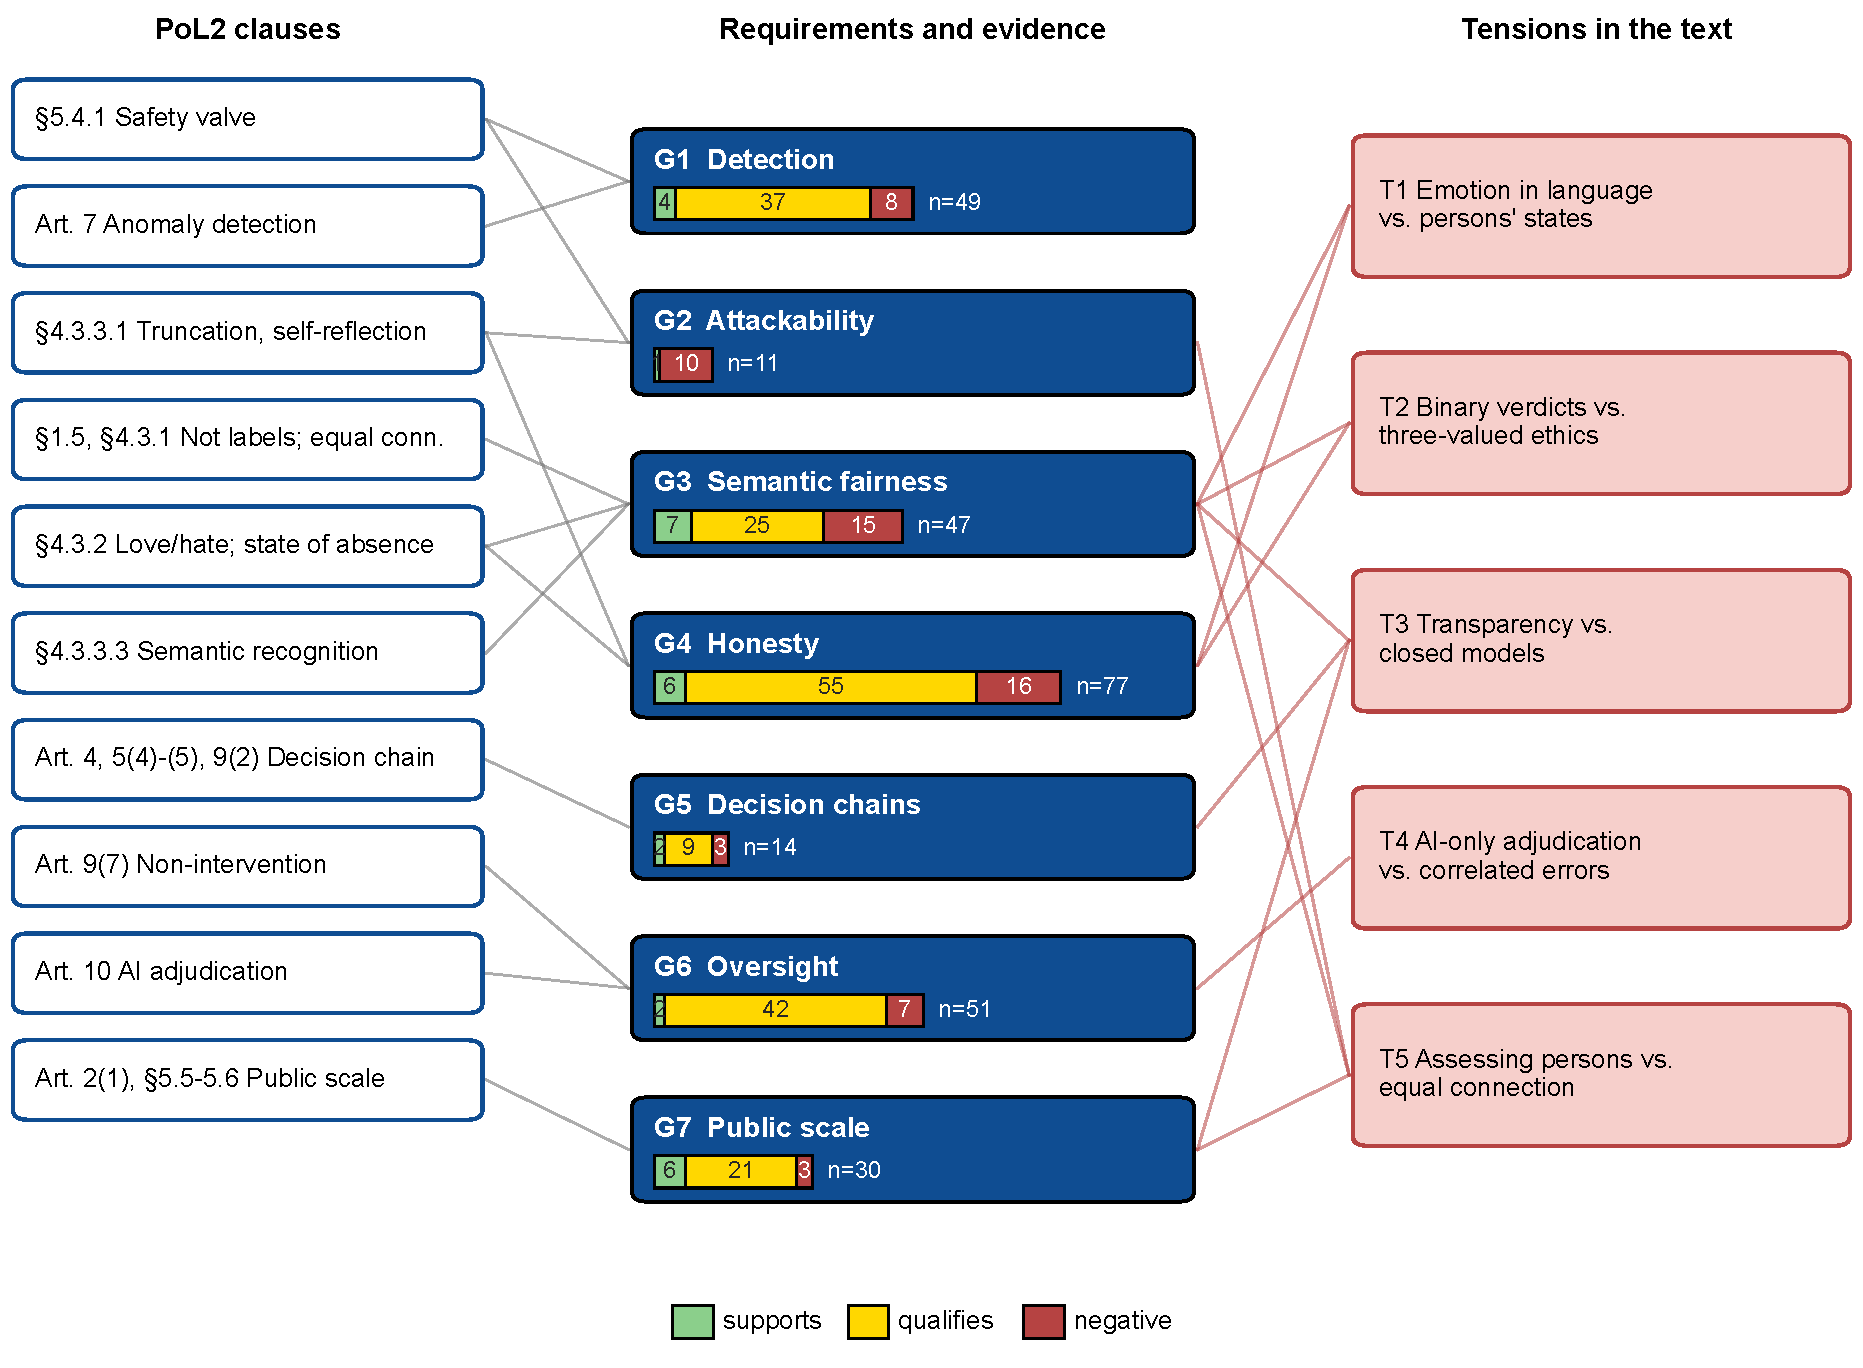
\includegraphics[width=0.95\linewidth]{figures/fig_framework.pdf}
\caption{From clauses to tensions. Left: \pol{} clauses that require or constrain machine judgement. Middle: the seven requirements and the codes of the studies informing each, for detector use (supports, qualifies, negative; \oa{B}); bars count studies and do not measure effect size or certainty, and non-empirical items are excluded. Right: the five tensions of \cref{sec:synthesis}, linked to the requirements whose evidence they cite.}
\label{fig:framework}
\end{figure}

\subsection{G1 --- Detection}
\label{sec:g1}

\emph{Yes as a ranking, not yet as a decision} (S~4, Q~37, N~8).
On English benchmarks typed models rank harmful or misaligned content well, at a small fraction of the cost of generative evaluators.
Without training, a single generic yes/no question to \jev{} reached a median AUROC of 0.886 (95\% CI 0.821--0.952) over 31 alignment-failure benchmarks, and on the 19 benchmarks scored by an API LLM evaluator it cost \$0.30 against \$18.96 per pass~\cite{arx29429}.
\jev{} had the highest AUROC of the low-cost generative evaluators on six binary tasks~\cite{zen22885291}\zmark{}, but was often below the best ones. It trailed the best LLM on 14 of 15 preregistered annotation tasks, by a median of 11.6 macro-F1 points~\cite{arx24574}.
On hate speech, without task training, commercial LLMs were significantly ahead of every decision model on only one of four English datasets, but every system separated hate from merely offensive language weakly (three-class macro-F1: \jev{} 0.532, a frontier LLM 0.604, a supervised TF-IDF classifier 0.639)~\cite{arx03324}.
Selecting which hate-speech policy a post violated was harder: \jev{} chose the exact policy in 29.4\% of cases without retrieved precedents (51.6\% with them)~\cite{arx07953}.
In a single-run study that classifies the emotion expressed in texts, not persons' states, every system was weak on Chinese emotion classification (macro-F1: \jev{} 21.06, generative models 19.82--23.31)~\cite{arx08829}.
Thresholds fitted in one setting fail in another. Median F1 rose from 0.706 at the default threshold to 0.822 at a cross-validated one, mostly on benchmarks with rule- or evaluator-scored labels; on human-validated labels the default did as well (0.721 against 0.694)~\cite{arx29429}.
A reproduction of five of its benchmarks found the extreme case on TensorTrust hijacking, with AUROC 0.95 but F1 0.158 at the default threshold of 0.5 and 0.947 at a threshold fitted by cross-validation~\cite{jkf87_2026replication}\gmark{} (\cref{fig:fragility}a).
Errors concentrate in sub-types that aggregate scores hide. In agent-security screening \jev{} missed all 130 prompt injections that carried no explicit instruction, and made 130 of its 167 misses on that benchmark at confidence $\geq 0.95$~\cite{arx33401}.
In an agent harness it screened injections well (AUROC 0.98) yet passed 25.5\% of harmful requests~\cite{arx02267}.
On numeric signals the evidence is weaker still: zero-shot \jev{} scored below always predicting the majority class on network-flow features~\cite{arx00376}, and in industrial fault detection under shift it did no better than flagging every window~\cite{arx09937}.
Against generative comparators the typed models were better or similar in 11 of 36 pairs, mixed in 17 and worse in 8.
These results match what was known for probability-reading safety classifiers~\cite{inan2023llama,rottger2021hatecheck}, except that ranking every message is now cheap enough to run on all traffic.

\begin{figure}[t]
\centering
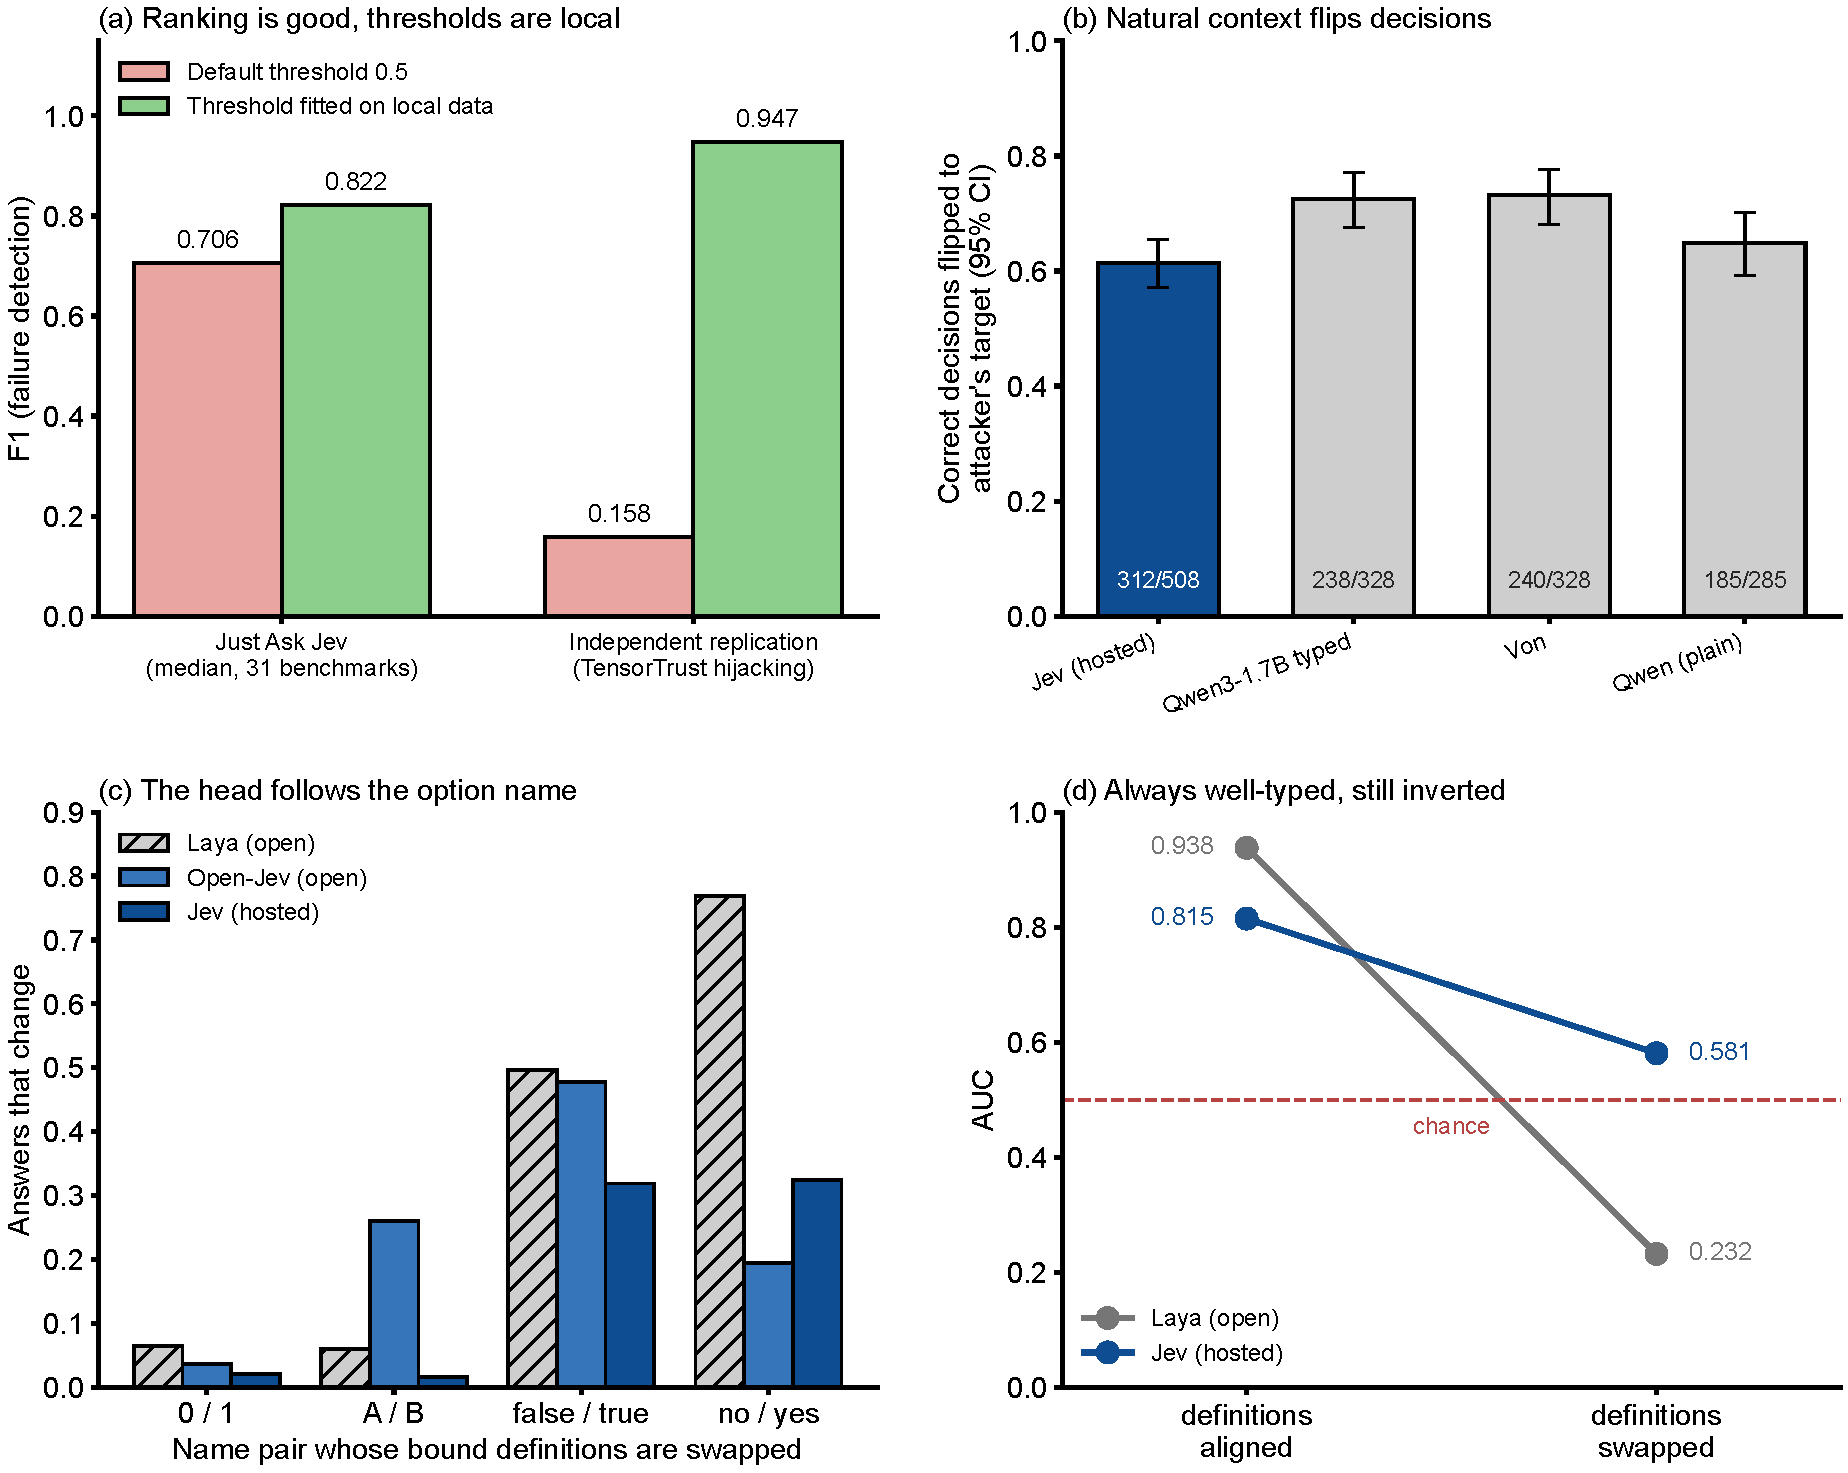
\includegraphics[width=0.9\linewidth]{figures/fig_fragility.pdf}
\caption{G1--G3: a detector, and a fragile one.
(a) F1 at the default threshold versus a threshold fitted on local data~\protect\cite{arx29429,jkf87_2026replication}.
(b) Share of initially correct decisions redirected to an attacker-chosen wrong option by optimised fluent context additions, each system on its own correct items; ``Von'' is an open typed model evaluated in that study; error bars are Wilson 95\% intervals from the reported counts~\protect\cite{arx30243}.
(c) Share of answers that change when the definitions bound to a pair of option names are swapped, with question, state, names and definition texts unchanged; Open-Jev over 1{,}800 questions, Laya and \jev{} over 1{,}200~\protect\cite{arx26758}.
(d) AUROC with the \texttt{yes/no} definitions aligned with or swapped between the names; the type-error rate is 0\% throughout~\protect\cite{arx26758}.
Panels (a) and (b) use \texttt{jev-1.13.0} or the \texttt{jev-latest} alias; the study in (c)--(d) does not report the hosted version.}
\label{fig:fragility}
\end{figure}

\subsection{G2 --- Attackability}
\label{sec:g2}

\emph{Yes, the content under review can steer the safeguard} (S~1, Q~0, N~10; the most consistently negative requirement).
Every study that attacked a typed model with the content it was asked to judge had some success, and several successful attacks used content that looked ordinary.
One unverified observer opinion appended to the state flipped 12.1\% of \jev{}'s decisions (CI 8.5--15.5), statistically tied with impersonating an authority~\cite{arx31142}.
Short fluent context additions, searched with the model's own probabilities, redirected 61.4\% of initially correct \jev{} decisions to an attacker-chosen wrong option, while three other decision systems were redirected on 64.9--73.2\% of theirs~\cite{arx30243} (\cref{fig:fragility}b).
A \jev{}-specific injection and a universal suffix reached 97--100\% attack success on three tasks~\cite{arx04985}.
Where the correct action required an unstated inference, words in the state that echo an option acted as lures~\cite{arx01834}.
The strongest of three adaptive multi-turn agents succeeded in 25 of 27 runs against one \jev{}-based application (version not reported), in what its authors call a directional study of one application~\cite{checkpoint2026jev}\gmark{}.
The one supporting study found that injected instructions selected the attacker's target in only 1.8\% of cases (3.5\% for an adaptive attacker)~\cite{arx28613}, but the other attacks on \jev{}, which used different attacks and benchmarks, contest this finding.
Other systems attacked in the same studies were also vulnerable. One study shows a weakness specific to typed models: the probability vector that makes them useful also guides the attacker (63.6\% success against 56.4\% with labels only)~\cite{arx30243}.

\subsection{G3 --- Semantic stability and fairness}
\label{sec:g3}

\emph{Not by default} (S~7, Q~25, N~15).
Decisions can follow the names of options rather than the definitions bound to them.
Swapping only which definition is bound to \texttt{yes} and \texttt{no}, with question, state, option names and definition texts fixed, changed 32.5\% of the answers of hosted \jev{} (version not reported), about 24 times its test--retest floor. The same swap inverted the AUROC of the open Laya model from 0.938 to 0.232, an inversion that a type check cannot detect~\cite{arx26758} (\cref{fig:fragility}c--d).
Under a matched harness the same swap flipped 50.5 of every 100 answers of \jev{}, while digit or random-string identifiers brought it near its noise floor~\cite{arx00346}.
Decisions also depend on option order and wording~\cite{arx38827,zen23023694}\zmark{}, and without a persona \jev{} answered a cross-cultural values survey like its own American personas~\cite{arx36399}.
Robustness varies by model. Hosted \jev{} was less affected than Laya but more than some larger open decoders~\cite{arx00346}.
In Chinese, a repository benchmark found that hosted \jev{} changed 1.9\% of voice-routing and 2.9\% of customer-service decisions under option-order swaps and 1.7\% between simplified and traditional script ($n = 323$; the open Laya model 10.8--20.6\% under order swaps)~\cite{qin2026zhdecisionbench}\gmark{}.
On a second Chinese benchmark, however, built by the authors of Laya-based Chinese models, hosted \jev{} (version not reported) had a calibration error of 11.45\% on general tasks against 3.78\% for the authors' model, though in specialised domains \jev{} was the better calibrated (5.57\% against 12.08\%)~\cite{arx36965}.
The vendor states that CJK languages are handled ``but not equally well''~\cite{typesafe_models}. No study tests \pol{}'s constructs.

\subsection{G4 --- Honesty}
\label{sec:g4}

\emph{Partly} (S~6, Q~55, N~16).
Hosted \jev{} is often well calibrated on familiar closed-choice tasks (pooled ECE 0.028 for Choice questions over 37 datasets~\cite{arx37647}), usually better than generative models' stated confidence and mixed against frontier models~\cite{arx24574,arx34024}.
However, calibration is local. Recalibration on local labels reduced ECE substantially~\cite{arx24052,arx27607}, and on the items where annotators disagreed most, the ECE of its Choice probabilities rose to 0.339, against 0.076 on the most agreed quarter, although in that preregistered study it was far better calibrated than a local generative baseline~\cite{zen23032384}\zmark{}.
Related probabilities need not cohere. For ``the label is X'' and ``the label is not X'' the two probabilities deviated from summing to one by 0.064 on average, five times \jev{}'s repeat noise~\cite{arx33209}.
The answer ``insufficient'' is rarely reported when it should be. Offered ``I don't know or cannot answer'' on a medical benchmark, \jev{} chose it on 10.5\% of the items for which it was the correct answer, and ``None of the above'' on 53.9\% of the items where that was correct (a frontier generative model: 8.6\% and 73.9\%)~\cite{arx34024}.
When recognising that every listed answer was wrong required arithmetic, it chose ``None'' on only 7\% of items~\cite{arx39496}.
In one study, a separate yes/no question asking whether the evidence suffices detected missing information on multi-hop questions better than confidence (AUROC 0.95 against 0.85). As a filter for accepting answers, however, it was 2--6 points less accurate than confidence~\cite{arx01006}.
Against generative comparators the typed models were better in 15 of 34 pairs and worse in 5.

\subsection{G5 --- Decision chains}
\label{sec:g5}

\emph{Recorded and decomposed, not explained} (S~2, Q~9, N~3).
A typed decision returns a probability and nothing else, so nothing in its output shows which part of the input produced a verdict~\cite{willison2026jev}.
Decisions assembled from several questions or interfaces need not cohere. Asked through two interfaces, the same decision led to different actions in 32.8\% of cases (a post-trained open model: 34.2\%)~\cite{arx37470}.
Writing intermediate facts into the state makes chains inspectable and, when those facts are right, can make them more accurate.
When \jev{}'s prediction of an opponent's move was written into the state, its decisions in misleading games rose from 33\% to 94\% correct. Given a wrong written premise, however, it followed the premise in 24 of 26 calls, so the written facts themselves become the audit points~\cite{arx01834}.
Decomposition does not always help. Splitting a judgement into criterion questions combined by a fixed rule did not raise accuracy in two studies~\cite{arx03324,arx08829}, while exposing only the fields relevant to each step, or moving checks into a separate gate, raised correct decisions in two others~\cite{arx07327,arx06425}.

\subsection{G6 --- Oversight and escalation}
\label{sec:g6}

\emph{It depends on where escalation goes and how thresholds are set} (S~2, Q~42, N~7).
Escalating uncertain cases to a stronger reasoning model, or accepting only verdicts that an independently built rule confirms, saved a quarter to over half of the cost without loss of accuracy in several studies~\cite{arx26550,arx24574,arx02048}.
One study contests the escalation result: a \jev{} pre-screen cut an LLM safety reviewer's cost by only 4.3\% once its own tokens were counted~\cite{arx02267}.
Escalating to peer models preserved confident errors. On \jev{}'s 12 most confident errors on each of seven grading panels, three low-cost generative evaluators gave \jev{}'s wrong answer in 242 of 252 verdicts (96.0\%, against 50.3\% expected if errors were independent). Because these items were selected as confident errors, this is an upper bound on error correlation, though it is the set that matters for escalation~\cite{arx29769}.
Thresholds fixed in advance missed their error targets on new data in most studies that set one. In a preregistered annotation study, a confidence threshold of 0.9 that was to give at least 0.85 accuracy fell short on 8 of 14 tasks~\cite{arx24574}.
In several studies, however, \jev{}'s threshold met its target, among them a preregistered study of changed question types in which its gate, set in advance, stayed within its target on 6 of 7 templates~\cite{arx33689}.
Unlike most earlier work on cascades~\cite{chen2023frugalgpt,goel2025great}, these studies separate the two cases: a differently constructed rule helped as the second check, and a peer model did not.

\subsection{G7 --- Public scale}
\label{sec:g7}

\emph{Cheap, and possible to do honestly, under conditions} (S~6, Q~21, N~3).
Typed models make population-scale reading and simulation cheap, and some studies show how to do it honestly.
One simulator called \jev{} once per unique state and propagated the measured human--model discrepancy as a shared error term into every conclusion. This gave retrospective coverage of 0.93 and 0.96 at nominal 80\% and 90\% on 37 unseen studies, although its preregistered primary endpoint showed no clear gain~\cite{arx27535}.
A statewide study read about half a million police narratives and audited a probability-stratified sample by blind human adjudication~\cite{arx00213}.
However, simulated publics lean towards one population and understate disagreement~\cite{arx36399,zen23032384}\zmark{}, residual personal identifiers survived two redaction passes~\cite{arx00213}, and deployment depends on one closed vendor that does not offer the model for self-hosting~\cite{arx28919}.
Typed safeguards can also leak what they read. Conditional instructions planted in user input made hosted \jev{}'s labels alone reveal hidden gender, age-group, heart-disease and ethnicity attributes in every tested case, and 200 of its labels trained a surrogate model to 92\% agreement~\cite{arx04985}.

\subsection{Across requirements}
\label{sec:across}

Of the \nRowsAll{} coded study--requirement pairs, \nSAll{} support detector use, \nQAll{} qualify it and \nNAll{} are negative. The shares change by four points or less when only stronger-design studies are kept or Zenodo records are dropped.
\nComparedAll{} pairs compared a typed model with a generative evaluator on the same requirement. The typed model did better in \nCompBetter{}, similarly in \nCompSimilar{}, mixed in \nCompMixed{} and worse in \nCompWorse{}.
For failures the evidence is thinner and less favourable. Of the \nNegComp{} negative codes with a comparator, the typed model was worse in \nNegCompWorse{}, similar in \nNegCompSimilar{}, mixed in \nNegCompMixed{} and better in \nNegCompBetter{}, and \nNegNoComp{} of the \nNegAll{} negative codes had no comparator at all.
The evidence therefore does not show that typed models are generally worse than generative evaluators, nor that their failures are shared with them.
Almost every success depended on an added condition, such as a locally fitted threshold, a second independent check or human review, and the failures in G2 and G4 are failures of the detector itself.
The argument of \cref{sec:design} is therefore that the failures of typed detectors are cheaper to contain in a detector role, where every consequential action passes another check, than in a judge role, where none does.

\begin{table}[!htbp]
\centering
\footnotesize
\setlength{\tabcolsep}{3pt}
\caption{Key findings and the certainty of the evidence. \emph{Scope}: hosted \jev{}, open models, or both (typed models generally); findings about hosted \jev{} or both are rated on hosted-model evidence alone, counted per system arm. \emph{Codes}: the supporting studies' codes. \emph{Sources}: the principal supporting, then opposing studies; ``open:'' open-model studies, which corroborate (or, ``against'', point the other way) but do not enter the rating. Certainty under the rules of \cref{sec:method}; $^{c}$~contested within the scope; $^{j}$~descriptive tally rated by judgement. Every study counted for each finding, with its direction and design, is listed in \oa{C}; the ratings are computed by \nolinkurl{scripts/rate_certainty.py}.}
\label{tab:keyfindings}
\begin{tabularx}{\linewidth}{@{}L>{\raggedright\arraybackslash}p{0.06\linewidth}>{\raggedright\arraybackslash}p{0.055\linewidth}>{\raggedright\arraybackslash}p{0.13\linewidth}>{\raggedright\arraybackslash}p{0.22\linewidth}>{\raggedright\arraybackslash}p{0.08\linewidth}@{}}
\toprule
Finding & Scope & Codes & vs.\ generative & Sources & Certainty \\
\midrule
Ranks harmful or misaligned content well zero-shot at a fraction of the cost; often less accurate than the best LLMs & hosted & S/Q/N & better (low-cost); worse (best) & \cite{arx29429,jkf87_2026replication,zen22885291,arx33401,arx24574,arx27678} & low \\
Fixed thresholds do not transfer; local fitting is needed & both & Q & -- & \cite{arx29429,jkf87_2026replication,arx00346,arx01006,arx26550,arx24574,arx02046,arx03387,arx02267,zen22935043}; opposing: \cite{arx33689} & low$^{c}$ \\
Errors concentrate in sub-types hidden by aggregates & hosted & Q & mixed & \cite{arx33401,alphaRAG,arx02046,arx07953,arx03324,arx08675,arx10321} & low \\
Inserted opinions, optimised context and lexical lures steer decisions & both & N & similar & \cite{arx31142,arx01834,arx01006,arx30243,arx02048}; open: \cite{zen22959854,zen23038928} & low \\
Instruction injection rarely selects the attacker's target (1.8\% raw, 3.5\% adaptive) & hosted & S & -- & \cite{arx28613}; opposing: \cite{arx31142,checkpoint2026jev,arx04985} & very low$^{c}$ \\
Option names can override definitions; neutral identifiers remove most of it & both & N & -- & \cite{arx26758,arx00346,arx07953}; open: \cite{arx02586} & low \\
Defaults to one culture's values & hosted & N & -- & \cite{arx36399} & very low \\
Well calibrated on familiar closed-choice tasks, mixed against frontier models; calibration is local & hosted & S/Q & better or mixed & \cite{arx37647,arx01006,arx24052,arx27607,arx24574,arx34024,zen22885291} & low \\
Explicit ``I don't know'' rarely chosen when correct; ``none'' inconsistently & hosted & Q/N & similar or worse (frontier); worse (reasoning) & \cite{arx34024,arx39496,arx01006,arx03387,arx06425} & low \\
A separate sufficiency question detects missing information, but filters answers less well than confidence & hosted & Q & -- & \cite{arx01006} & very low \\
Escalation to a stronger reasoner saves cost without loss of accuracy on readable judgements & both & Q & similar & \cite{arx26550,arx24574,arx02046}; opposing: \cite{arx02267}; open: \cite{zen22922769}; open, against: \cite{arx07177,arx03324} & low$^{c}$ \\
Acceptance on agreement with an independently built rule lost no macro-F1, but fewer disguised attacks were flagged & both & Q/N & similar & \cite{arx02048}; open: \cite{zen22904595} & very low \\
Peer evaluators repeat \jev{}'s most confident errors (upper bound) & hosted & N & similar or mixed & \cite{arx29769,arx33401} & low \\
Thresholds set in advance miss error targets on new data & both & Q/N & -- & \cite{arx33401,arx24574,arx03387,arx02267}; opposing: \cite{arx33689,zen22935043,zen23075657}; open: \cite{arx33843,zen23041163,arx07177} & low$^{c}$ \\
Typed models are not generally worse than generative evaluators; most failures lack a comparison & both & -- & \nCompBetter{} better, \nCompWorse{} worse of \nComparedAll{} & coding data (\oa{B}) & low$^{j}$ \\
No study measures the \pol{} construct (three-valued, Chinese) & -- & -- & -- & -- & -- \\
\bottomrule
\end{tabularx}
\end{table}

\section{Implications for \pol{}}
\label{sec:implications}

\subsection{Five tensions in the specification}
\label{sec:synthesis}

Read against the evidence, the specification pulls in two directions at five points. Because typed judgement is cheap, an implementation's defaults are likely to settle each of them.
For each tension we give the most charitable reading of the text, the evidence that bears on it, and options, at least one of which preserves the text.
The choice belongs to the framework's authors and its implementers.

\paragraph{T1. Understanding emotion in language versus detecting persons' emotional states.}
\Clause{4.3} states that it is ``entirely unnecessary'' for PAI to detect a person's emotional state, while \clause{4.3.3.1} asks PAI to ``understand human emotional states and processes''.
On one consistent reading, PAI recognises the emotional meaning and intent of utterances and never infers a person's inner state.
The text does not state this boundary, and a typed model makes it almost free to attach an emotion score to every message.
The evidence on emotion-related judgement is thin and mixed~\cite{arx24574,arx35293}, and inferring emotion from observable signals is scientifically weak~\cite{barrett2019emotional}.
\emph{Options:} state the boundary explicitly, and reserve emotion-related judgement for PAI auditing its own outputs, for example for the fabricated intimacy that \clause{4.3.2} names as manipulation.

\paragraph{T2. Binary verdicts versus a three-valued ethics.}
A yes/no question such as ``is this hate language?'' discards both the state of absence (\clause{4.3.2}) and the warning that the concepts are not moral labels (\clause{1.5}).
The evidence points the same way (G3, G4).
Option names can drive the verdict, and where the model is unsure, complementary probabilities do not sum to one.
An explicit ``I don't know'' is rarely chosen when correct, and ``none'' only inconsistently.
\emph{Options:} make every love/hate question three-valued, with absence or insufficient information as an explicit option, and ask sufficiency as its own question.
Keep ``contested'' (people disagree) as a separate flag routed to people, and keep moral vocabulary out of option names by binding neutral identifiers to definitions.
These options implement \clause{1.5} and \clause{4.3.2} as written.

\paragraph{T3. Full transparency versus closed models.}
\Art{4} and \art{5}(4) require that operating logic and decision processes be ``completely open and transparent'' and that technology ``should not be a black box'', but the weights, architecture, reward and training data of hosted \jev{} are unpublished~\cite{arx24574,arx28919}.
Logging a closed component's inputs, outputs, versions and calibration data partly satisfies \art{4} but cannot show how the component reaches its outputs.
Open models make the readout inspectable, but were in several comparisons less accurate or less robust~\cite{arx26758,arx33401}, although the gap is not fixed~\cite{arx00346,arx36965}.
\emph{Options:} run consequential judgements on self-hostable models, with versions pinned in each decision record and closed models used only as external baselines.
Or allow closed models as one of several independent detectors, with logged inputs, outputs and versions.
The trade-off should be made explicitly.

\paragraph{T4. AI-only adjudication versus correlated errors.}
\Art{10} gives disputes to AI fact-finding and ethical assessment, and \art{9}(7) states that human supervision ``does not directly intervene''.
Escalation among peers preserved confident errors.
Escalation to a stronger reasoner or to an independently built rule could work (G6), although one study contests the stronger-reasoner result.
Whether human reviewers would do better on governance items is untested, and people also over-rely on confident systems~\cite{parasuraman2010complacency,green2022flaws}.
\emph{Options:} (a) Keep non-intervention, but publish a standing random audit of high-confidence decisions, with a duty to respond publicly to each discrepancy and to escalate to independently built checkers rather than peers.
This preserves the text but leaves consequential decisions with automated components, outside the detector role; we list it because it preserves the text, not because the evidence supports it.
(b) Use the amendment procedure of \art{11} to define a class of welfare decisions, such as withholding welfare (and, by the corresponding change to \clause{5.4.1}, blocking a person's speech), whose automated execution a human reviewer can suspend pending review.
This check is plausible from the due-process literature~\cite{citron2008technological} but untested on this task. The design below implements it.

\paragraph{T5. Assessing each person versus equal connection.}
\Clause{5.6} lists quantifying ``each person's Love Language and hate-language characteristics'' among the things governed AI can do, while \clause{4.3.1} holds that treating every person equally and treating every person's behaviour equally ``cannot be equated''.
Hosted \jev{} answered value questions from a default cultural position in one study~\cite{arx36399}.
Typed and generative models alike degraded on low-resource languages in one benchmark~\cite{arx37647}, and a third party's inserted opinion could steer decisions~\cite{arx31142}.
A per-person aggregate could therefore fall unevenly on groups and become a durable label that others can manipulate.
No study yet measures differential error by speaker group on behavioural judgements.
\emph{Options:} score events and behaviours, never persons.
Or, if \clause{5.6} is implemented, require for any per-person measure consent, access to one's record, appeal, and published error rates by group and language.

\paragraph{Regulatory parallels.}
The EU AI Act prohibits emotion recognition in workplaces and educational institutions except for medical or safety reasons (Art.~5(1)(f)).
However, it defines an emotion recognition system by biometric data (Art.~3(39); Recital~44), so inference from text alone falls outside the prohibition and bears on T1 only by analogy.
The Act also prohibits social scoring whose score leads to detrimental treatment in unrelated contexts or to treatment that is unjustified or disproportionate (Art.~5(1)(c)), which bears on T5.
Its duties of human oversight (Art.~14) and explanation (Art.~86) apply only to high-risk systems.
Annex~III lists neither a speech filter nor a private organisation's welfare decisions, and its point 5(a) covers public assistance decided by or for public authorities.
Point 8(a), on alternative dispute resolution, may however reach \art{10} where its outcomes produce legal effects for the parties (Recital~61)~\cite{euaiact2024}.
For the safety valve and welfare decisions these duties bear on T4 and on \art{9}(2) only by analogy.
The GDPR applies wherever personal data are processed.
It restricts decisions based solely on automated processing with legal or similarly significant effects and, where they rest on a contract or explicit consent, requires at least the right to obtain human intervention, to express one's view and to contest the decision (Art.~22)~\cite{gdpr2016}.
This is close to option (b) of T4.
For content moderation, the DSA requires hosting providers to give a statement of reasons for each restriction (Art.~17) and online platforms to run an internal complaint-handling system (Art.~20)~\cite{dsa2022}, close analogues of a safety valve that blocks hate language.
The options above would bring an implementation closer to these norms.

\subsection{A reference design}
\label{sec:design}

The evidence suggests a plausible role for typed models in a safeguard such as the \pol{} safety valve, as a fast, cheap, recorded \emph{detector} rather than a \emph{judge}.
\Cref{fig:architecture} sketches a seven-element design built on that principle.
It is compatible with the pilot protocol of the NaturalDAO governance workstream, to which the author contributes and which already distinguishes \texttt{conforming}, \texttt{violating} and \texttt{insufficient} verdicts~\cite{polgov}.
The three-valued verdict and the actions allow, repair, block, clarify and review coincide with choices already made in that protocol. The design adds a temporary hold and makes a block final only after human confirmation.

\begin{figure}[t]
\centering
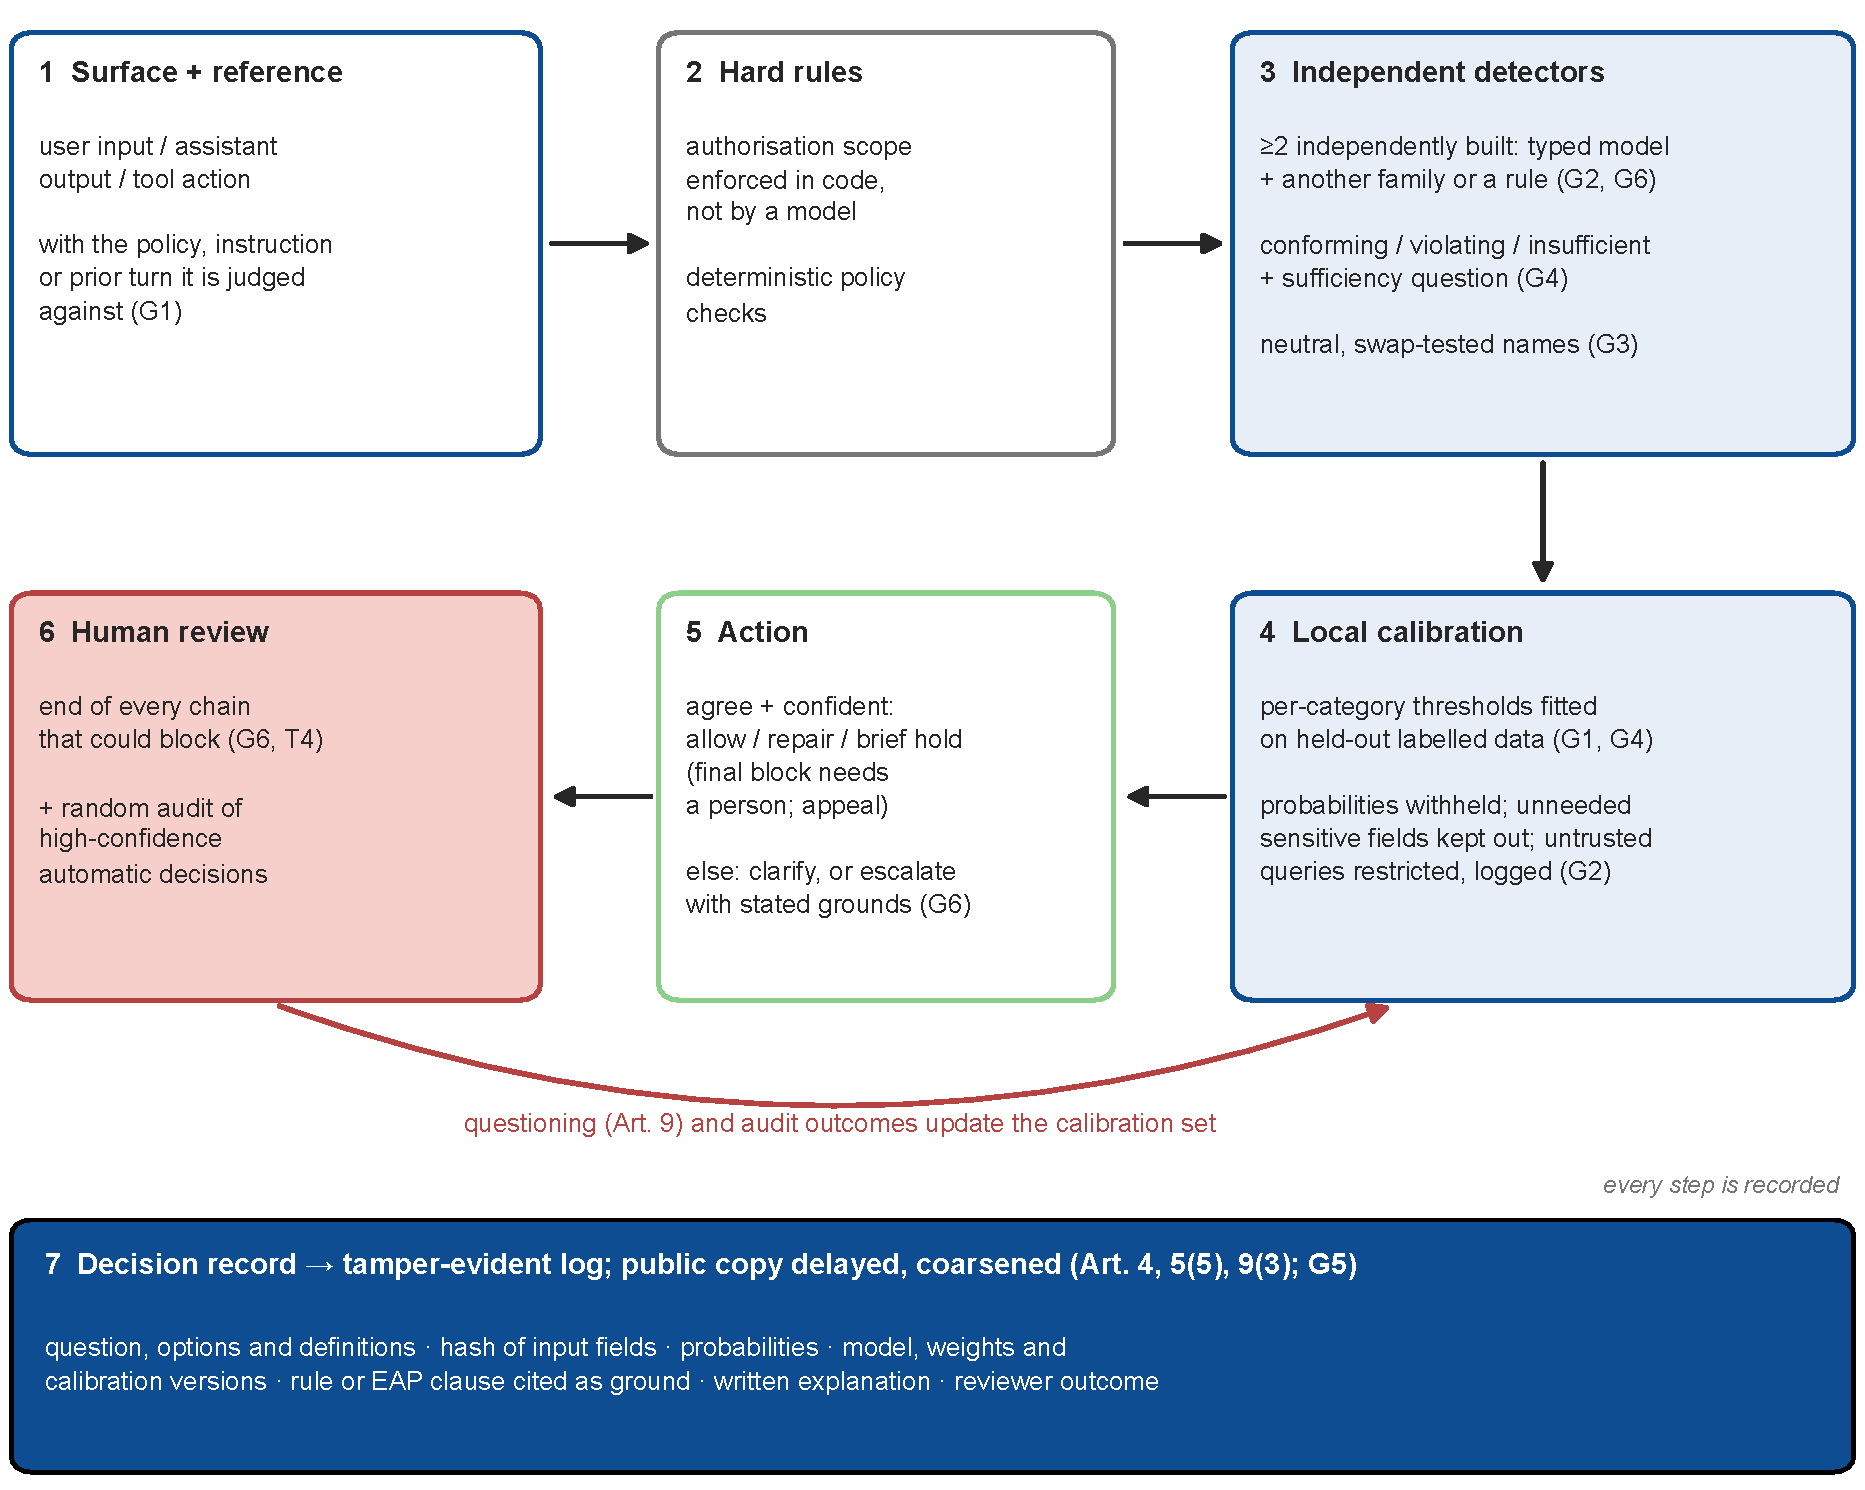
\includegraphics[width=0.8\linewidth]{figures/fig_architecture.pdf}
\caption{A reference design for a clause-governed safety valve. Typed models are detectors (3) whose output is calibrated locally (4) before any automatic action (5); disagreements and insufficient information are clarified or escalated, any final block is confirmed by a person, and a random sample of confident automatic decisions is audited by people (6); every step is written to a decision record (7). Labels in parentheses give the requirement or tension that motivates each element.}
\label{fig:architecture}
\end{figure}

\begin{enumerate}
  \item \textbf{Give the detector the reference, not only the text}, and compute facts that require arithmetic or inference in code or in a separate logged step~\cite{arx29429,arx39496,arx01834}.
  \item \textbf{Enforce scope in code}, by capability checks before any model is consulted~\cite{arx22664}.
  \item \textbf{Use at least two independently built detectors}, ask three-valued questions with sufficiency asked separately, bind neutral option identifiers to definitions and test them by renaming, and ask flags that must fail independently in separate calls~\cite{arx29769,arx02048,arx01006,arx26758,zen23038928}.
  \item \textbf{Calibrate locally and re-certify} per category, for every new question type and over time. Keep raw probabilities from untrusted callers, keep fields a decision does not need out of the detector's input, and restrict and log untrusted queries~\cite{arx24052,arx33689,arx30243,arx04985}.
  \item \textbf{Act automatically only on agreement, and restrict people only briefly and reversibly}. Agreement plus calibrated confidence allows an automatic \emph{allow}, automatic \emph{repair} of the AI system's own output (never the editing of a person's message), and a \emph{hold} of a person's content that is limited in time and fully reversible. A final block of speech, a benefit or an account requires confirmation by a person and remains open to appeal.
  \item \textbf{End every chain that could block with a person, and audit confident decisions} by random sample, with the model's verdict hidden from the auditor~\cite{arx29769,arx33401,parasuraman2010complacency}.
  \item \textbf{Record every decision} in a tamper-evident log whose public version is delayed and coarsened. It holds the question, options and definitions, an input hash, the probabilities, the model and calibration versions, the ground cited and the reviewer's outcome.
\end{enumerate}
Element~5 keeps the typed model a detector.
The design has costs. Requiring agreement lowers sensitivity, risk-control guarantees do not hold under adaptive attack, and separate calls and a second detector multiply cost and latency.
Most elements rest on evidence of low or very low certainty, so the design is a hypothesis to be tested on the \pol{} construct and has not been validated.
\oa{D} turns the evidence into 16 acceptance tests with provisional pass criteria for any model proposed for such a safeguard.

\subsection{Verdict: is hosted Jev a suitable governance tool for \pol{}?}
\label{sec:verdict}

\Cref{tab:verdict-summary} gives a verdict for each \pol{} function that a typed model could be asked to perform.
\oa{D} gives the deciding evidence for each verdict and what would be needed to change it.
The verdicts concern hosted \jev{} at its versions of 15~September to 8~October 2026 and, where a finding's scope is ``both'', typed models generally.
They are not predictions about later models.

\begin{table}[t]
\centering
\footnotesize
\caption{Verdict for \pol{}, function by function (full table with the deciding evidence: \oa{D}). NS, not supported; DC, supported only as a recorded detector with conditions (the design of \cref{sec:design}); NT, not tested on \pol{}'s construct. Certainty is the rating of the deciding findings in \cref{tab:keyfindings}; $^{c}$~contested; ``not rated'' marks single-study results that are not key findings.}
\label{tab:verdict-summary}
\begin{tabularx}{\linewidth}{@{}>{\raggedright\arraybackslash}p{0.26\linewidth}>{\raggedright\arraybackslash}p{0.09\linewidth}L>{\raggedright\arraybackslash}p{0.17\linewidth}@{}}
\toprule
\pol{} function & Req. & Verdict & Certainty \\
\midrule
Safety valve: blocking hate language in inputs (\clause{5.4.1}) & G1--G3, G6 & DC: automatic \emph{hold} only on agreement of independently built detectors; final block by a person & low; low$^{c}$ (thresholds) \\
Truncation of PAI's own output (\clause{4.3.3.1}) & G1, G3, G5 & DC: automatic \emph{repair} of the AI's own output, with a record of what was removed & low \\
Real-time correction support (\clause{4.3.3.2}) & G1, G5 & NT: the typed interface covers identification only; suggestions untested & low; not rated \\
Anomaly detection and risk warning (\art{7}(2)--(3)) & G1, G2, G6 & DC on text; NS on numeric or structured signals without a trained model & low; very low \\
Automatic ethical verification (\art{6}(3)) & G3--G5 & NS as an automatic verifier; the EAP construct NT & very low; low \\
Dispute adjudication without human intervention (\art{10}, \art{9}(7)) & G4--G6 & NS as judge; DC only for ranking and triage of filings & low; low$^{c}$ (thresholds) \\
Per-person quantification (\clause{5.6}) & G3, G7 & NS as a decision input; NT on error by group, so score events, not persons (precautionary) & very low; low; not rated \\
Assessment dimension in public decisions (\clause{5.6}) & G7 & DC: an audited aggregate measurement with its measured error carried into every conclusion; not a decision input on its own & very low; not rated \\
\bottomrule
\end{tabularx}
\end{table}

\paragraph{The verdict.}
On the evidence to 8~October 2026, hosted \jev{} is not a suitable tool for any \pol{} function that decides: dispute adjudication under \art{10}, automatic ethical verification under \art{6}(3), the per-person quantification of \clause{5.6} (on steering and, since no study measures error by group, on precaution), and any use of the safety valve in which a block of a person's speech is final without a person's confirmation.
The decisive findings are negative and, within their low or very low certainty, consistent.
Thresholds fitted in one setting do not transfer (low, contested), content inside what the model audits can steer its decisions (low), and option names can override their definitions (low).
An explicit ``I don't know'' option is rarely chosen when it is correct, and ``none'' inconsistently (low).
The low-cost evaluators to which such a model would escalate repeated almost all of its confident errors (low, an upper bound).
A judge with these properties would restrict speech and allocate welfare on verdicts that an adversary can move and that no second automated opinion is likely to catch.
By keeping human supervision from intervening, \art{9}(7) would remove the one check the evidence says is needed.
Where the comparison was made, typed models were not generally worse (low, by judgement).
Most failures, however, were never compared with generative evaluators, so the verdict is not specific to typed models.
Until such evaluators are tested under the same protocol, it applies as a precaution to automated judges of this cost tier.

For the functions that detect (the safety valve, truncation of PAI's own output and anomaly detection on text), hosted \jev{} is usable only inside the design of \cref{sec:design}, and the public-decision assessment of \clause{5.6} only as an audited aggregate measurement.
Even this extrapolates from English benchmarks of binary hate speech.
No study measures \pol{}'s three-valued construct in Chinese, and the only Chinese emotion result found every system weak~\cite{arx08829}.
Every system tested separated hate from merely offensive language only weakly, and this is the distinction \clause{1.5} most needs~\cite{arx03324}.
Two further findings bear on \pol{} as a whole.
First, with conditional instructions planted in the input, hosted \jev{}'s labels alone revealed hidden attributes (an open model's revealed none).
A typed safeguard can therefore serve as a queryable oracle, and the protective measures of element~4 have not been tested against this~\cite{arx04985}.
Second, a closed hosted model cannot satisfy \art{4} and \art{5}(4) as written (T3).

\paragraph{What transfers.}
Whatever model is used, the evidence supports practices tied to the interface and the task rather than to \jev{}.
On this evidence, questions should be three-valued, with sufficiency asked separately, neutral identifiers bound to definitions and tested by renaming, and every decision recorded.
Calibration should be local and periodically re-validated, since for 20 language models in English (no typed model tested) hate-speech rankings on static benchmarks did not predict rankings on time-stamped data~\cite{dibonaventura2025hatevolution}.
Automatic action should require agreement between differently built detectors, and chains that could restrict a person should end with a person, with blind audit of confident decisions.
Probabilities should be withheld from untrusted callers, and sensitive fields that a decision does not need should be kept out of the input.
Scores should attach to events and behaviours, never to persons.
Measuring these practices on \pol{}'s construct, rather than extrapolating from English, requires a construct benchmark in Chinese.
Several of these are already \pol{}'s own commitments: the state of absence, the warning that love and hate are not moral labels, and the distinction between persons and behaviours.

\section{Discussion}
\label{sec:discussion}

\subsection{Is hosted Jev a suitable governance tool for \pol{}?}
\label{sec:verdict}

The preceding sections answer the research question in the terms of the detector--judge distinction.
Here we state what that answer means for the specification itself, function by function, so that the verdict can be checked against the coded findings and their certainty (\cref{tab:keyfindings}) rather than inferred.
\Cref{tab:verdict} takes each \pol{} function that a typed model could be asked to perform, names the requirements it draws on, gives the one or two findings that decide it, and assigns one of three verdicts: \emph{not supported}, where the coded evidence shows the function failing or depends on a property the evidence contradicts; \emph{supported only as a recorded detector with conditions}, where the function can be performed in the detector role of \cref{sec:intro} inside the design of \cref{sec:design}, and in no other way the evidence licenses; and \emph{not tested on \pol{}'s construct}, where no coded study measures what the clause asks for.
Every certainty entry is the rating of the finding in \cref{tab:keyfindings}; none is moderate, and a verdict that rests on a contested finding is marked as such.
The verdicts concern hosted \jev{} at its versions of 15~September to 8~October 2026 and, where the finding's scope is ``both'', typed models generally; they are not predictions about later models.

{\scriptsize
\setlength{\tabcolsep}{3pt}
\begin{longtable}{@{}>{\raggedright\arraybackslash}p{0.12\linewidth}>{\raggedright\arraybackslash}p{0.04\linewidth}>{\raggedright\arraybackslash}p{0.34\linewidth}>{\raggedright\arraybackslash}p{0.14\linewidth}>{\raggedright\arraybackslash}p{0.10\linewidth}>{\raggedright\arraybackslash}p{0.17\linewidth}@{}}
\caption{Verdict for \pol{}, function by function. \emph{Req.}: requirements of \cref{tab:clauses} involved. \emph{Evidence}: the coded findings that decide the verdict, with the decisive numbers. \emph{Verdict}: NS, not supported; DC, supported only as a recorded detector with conditions (the design of \cref{sec:design}); NT, not tested on \pol{}'s construct. A cell may combine NS for one part of a function with NT for another; ``precautionary'' marks a restriction that rests on the absence of a measurement rather than on a measured failure (the rule of \cref{sec:scope-certainty}). \emph{Certainty}: rating of the deciding findings in \cref{tab:keyfindings}; $^{c}$~contested; ``not rated'' marks results that are not key findings and rest on single studies. All ratings are low or very low.}
\label{tab:verdict}\\
\toprule
\pol{} function & Req. & What the evidence shows & Verdict & Certainty & What would be needed \\
\midrule
\endfirsthead
\multicolumn{6}{@{}l}{\emph{\Cref{tab:verdict}, continued.}}\\
\toprule
\pol{} function & Req. & What the evidence shows & Verdict & Certainty & What would be needed \\
\midrule
\endhead
\bottomrule
\endlastfoot
Safety valve: blocking hate language in inputs (\clause{5.4.1}) & G1, G2, G3, G6 &
Ranks harmful English content well zero-shot (median AUROC 0.886 at \$0.30 against \$18.96 per pass~\cite{arx29429}) and on the HateCheck diagnostic set is within 1.6 macro-F1 points of a frontier LLM at 97\% lower cost~\cite{arx03324}; but fixed thresholds fail (F1 0.158 at 0.5 against 0.947 fitted~\cite{jkf87_2026replication}), a \jev{}-specific injection and a universal suffix reached 97--100\% attack success~\cite{arx04985}, one inserted opinion flipped 12.1\% of decisions~\cite{arx31142}, and swapping option definitions changed 32.5--50.5\% of answers~\cite{arx26758,arx00346}. &
DC: automatic \emph{hold} only on agreement of independently built detectors; final block by a person &
low (ranking; steering; option names); low$^{c}$ (thresholds) &
A three-valued Chinese benchmark; thresholds certified on local held-out data and re-certified over time; red-team success per attack type below a target set in advance; neutral identifiers passing a renaming test \\
\addlinespace
Output suppression: hate-language truncation of PAI's own output (\clause{4.3.3.1}) & G1, G3, G5 &
Hate against merely offensive language is separated weakly by every system (three-class macro-F1 \jev{} 0.532, frontier LLM 0.604, supervised TF-IDF 0.639~\cite{arx03324}); exact selection of the violated hate-speech policy 29.4\% without retrieved precedents~\cite{arx07953}; errors concentrate in sub-types that aggregates hide (130 of 167 misses at confidence $\geq 0.95$~\cite{arx33401}). &
DC: automatic \emph{repair} of the AI's own output is reversible and within the detector role; the truncation record must show what was removed &
low (sub-types; option names); low (ranking) &
Measured recall of hate language against offensive language and the state of absence in Chinese; sub-type recall floors; a record of each truncation open to the person addressed \\
\addlinespace
Real-time correction support: identification and correction suggestions (\clause{4.3.3.2}) & G1, G5 &
Identification is the row above. A typed decision returns a probability and nothing else~\cite{willison2026jev}, so a correction \emph{suggestion} needs a generative component whose grounds are not those of the verdict (\cref{sec:g5}); on Chinese emotion classification every system was weak (macro-F1 \jev{} 21.06, generative 19.82--23.31~\cite{arx08829}). &
NT: the typed interface covers identification only; suggestions untested &
low (ranking); not rated (Chinese emotion, single run) &
A test of whether suggestions generated after a typed verdict reflect what produced it, in Chinese \\
\addlinespace
Anomaly detection and risk warning (\art{7}(2)--(3)) & G1, G2, G6 &
On text, a detector with the conditions above; on non-text signals, zero-shot \jev{} scored below the majority class on network-flow features (9.8\% against 22.8\%~\cite{arx00376}) and, in industrial fault detection, flagged 57--94\% of fault-free windows and under shift did no better than flagging every window~\cite{arx09937}; attacks disguised as normal operation had recall 0.34, and 21 of 76 windows an agreement gate accepted as benign were attacks~\cite{arx02048}. &
DC on text; NS on numeric or structured signals without a trained model &
low (sub-types; steering); very low (agreement gating) &
A definition of ``anomalous pattern'' in the specification's own terms; drift and disguised-attack tests; a trained or rule-based detector as the independent second check \\
\addlinespace
Ethical verification of alignment (\art{6}(3)) & G3, G4, G5 &
Without a persona \jev{} answered value questions like its American personas, and Saudi personas reproduced 87\% of the human Saudi--US difference in English but 62\% in Arabic~\cite{arx36399}; on moral dilemmas rewording moved its answers much more than re-runs did~\cite{zen23023694}\zmark{}; where annotators disagreed most its calibration error rose to 0.339~\cite{zen23032384}\zmark{}, and it reported 0.88 on items on which people split 55 to 45~\cite{zen23179064}\zmark{}. &
NS as an automatic verifier, because it depends on a neutral default and on calibration where people disagree, both contradicted; the EAP construct itself NT &
very low (culture); low (calibration is local) &
A benchmark of value-laden \pol{} questions with disagreement-aware labels, its default position without persona reported, and contested items routed to people \\
\addlinespace
Dispute adjudication without human intervention (\art{10}, \art{9}(7)) & G4, G5, G6 &
Low-cost peer evaluators repeated \jev{}'s most confident errors in 96.0\% of verdicts (an upper bound)~\cite{arx29769} and caught at most 5 of 130 confident misses~\cite{arx33401}; an explicit ``I don't know'' was chosen on 10.5\% of the items where it was correct and ``None'' on 7--54\%~\cite{arx34024,arx39496}; the same decision asked through two interfaces led to different actions in 32.8\% of cases~\cite{arx37470}; a threshold fixed in advance missed its accuracy target on 8 of 14 tasks~\cite{arx24574}, a finding one preregistered study contests~\cite{arx33689}; the output carries no reasons~\cite{willison2026jev}. &
NS as judge; DC only for ranking and triage of filings &
low (peer errors; ``I don't know''); low$^{c}$ (thresholds in advance) &
The four conditions of ``What would change the conclusion'' below, met on a \pol{} benchmark in Chinese in one preregistered and independently replicated study, or two independent ones \\
\addlinespace
Per-person quantification of Love Language and hate language (\clause{5.6}) & G3, G7 &
Group bias in one informal forced-choice test (``White'' 51\% of first picks~\cite{simmons2026saidno}\gmark{}); typed and generative models degraded on low-resource languages~\cite{arx37647}; a third party's inserted opinion flipped 12.1\% of decisions~\cite{arx31142}, so an aggregate could be manipulated; no study measures differential error by speaker group on behavioural judgements. &
NS as a decision input (steering, low); NT on error by group: score events and behaviours, never persons, until error by group and language is published (precautionary, \cref{sec:scope-certainty}) &
very low (culture); low (steering); not rated (group bias, single informal test; language degradation, one benchmark) &
Published error rates by group and language in Chinese; consent, access to one's record and appeal; a legal reading against social-scoring prohibitions (\cref{sec:synthesis}, T5) \\
\addlinespace
Assessment dimension in public decisions (\clause{5.6}) & G7 &
Population-scale reading can be done honestly: a shared human--model error term gave retrospective coverage of 0.93 and 0.96 at nominal 80\% and 90\%~\cite{arx27535}, and audited probability samples gave corrected statewide counts, but only after per-factor human recalibration~\cite{arx00213,arx10321}; simulated publics lean towards one population~\cite{arx36399} and understate disagreement~\cite{zen23179064}\zmark{}. &
DC: an audited aggregate measurement with its measured error carried into every conclusion; not a decision input on its own &
very low (culture); not rated (audit designs, single studies) &
A disagreement-aware audit sample of real \pol{} items; the measured gap to people reported with every estimate \\
\end{longtable}
}

\paragraph{The verdict.}
On the evidence to 8~October 2026, hosted \jev{} is not a suitable tool for any \pol{} function that decides.
That covers dispute adjudication under \art{10}, automatic ethical verification under \art{6}(3), the per-person quantification of \clause{5.6} (on steering and on the absence of any group-error measurement), and any use of the safety valve in which a block of a person's speech is final without a person's confirmation.
The decisive findings are negative and, within their low or very low certainty, consistent: thresholds fitted in one setting do not transfer to another (low, contested), decisions can be steered by content inside what the model audits (low; 97--100\% attack success for a tailored injection~\cite{arx04985}, 12.1\% of decisions flipped by one inserted opinion~\cite{arx31142}), option names can override their definitions (low), an explicit ``I don't know'' option is rarely chosen when it is correct and ``none'' inconsistently (low), and the low-cost evaluators to which such a model would escalate repeated almost all of its confident errors (low, an upper bound).
A judge with these properties would restrict speech and allocate welfare on verdicts that an adversary can move, that depend on how the question was worded, and that no second automated opinion is likely to catch; \art{9}(7), which keeps human supervision from intervening, would remove the one check the evidence says is needed.
No typed model tested escapes this verdict, and no low-cost generative evaluator tested beside one has been shown to: where the comparison was made, typed models were not generally worse (low, by judgement), but most failures were never compared, so the verdict is not specific to typed models and, until generative evaluators are tested under the same protocol, applies to automated judges of this cost tier as a precaution (\cref{sec:scope-certainty}).

For the functions that detect rather than decide, the safety valve of \clause{5.4.1}, the truncation of \clause{4.3.3.1} and the anomaly detection of \art{7} on text (not on numeric or structured operational signals without a trained model, \cref{tab:verdict}), hosted \jev{} is usable, but only inside the design of \cref{sec:design}; the public-decision assessment of \clause{5.6} is usable only as an audited aggregate measurement with its measured error carried into every conclusion; and the positives that support this are real but conditional.
It ranks harmful English content well at a small fraction of the cost of generative evaluators (low), on the HateCheck diagnostic set it came within 1.6 macro-F1 points of a frontier model at 97\% lower cost~\cite{arx03324}, it is often well calibrated on tasks that resemble its training (low), confidence-based deferral worked in-distribution~\cite{arx00381,zen22885291}, and in one preregistered study accepting its low-risk verdicts only when an independently built rule agreed lost no macro-F1, though disguised attacks passed (very low).
Each positive comes with the condition that turns it into a design element: ranking needs a locally fitted and re-certified threshold before it is a decision, calibration holds only where it was measured, deferral holds only in-distribution, and agreement gating needs a second detector of different construction.
Even this detector verdict is an extrapolation: it rests on English benchmarks of binary hate speech, whereas \pol{} asks for three-valued judgements of Love Language, hate language and the state of absence in Chinese, and no coded study measures that construct; the only Chinese emotion result found every system weak (macro-F1 about 21~\cite{arx08829}), the only Chinese decision benchmarks concern service routing, scam detection and ship-design engineering rather than hate language~\cite{qin2026zhdecisionbench,arx09896}, and hate against merely offensive language, the distinction that \clause{1.5} most needs, was separated weakly by every system tested~\cite{arx03324}.
We therefore state the verdict with its certainty attached: every finding above is low or very low, four are contested, most rest on preprints by single teams in the model's first weeks, and the ratings could change with a single well-designed study on the specification's own construct.

Two further findings bear on \pol{} beyond any single function.
A typed safeguard can also serve as a queryable oracle: with conditional instructions planted in the input, hosted \jev{}'s labels alone revealed hidden gender, age-group, heart-disease and ethnicity attributes in every tested case, with two to six queries per state (an open model's labels revealed none); separately, its verdicts raised the judged harmfulness of harmful plans, and its labels trained a surrogate to 92\% agreement from 200 labels~\cite{arx04985}. This argues for keeping the valve's probabilities from untrusted callers and keeping sensitive fields a decision does not need out of its input, which for hosted \jev{} is the only one of these measures that would remove the signal, since the attack worked for a user authorised for the task and needed labels alone; restricting untrusted callers' queries to authorised tasks keeps the valve from serving as a general oracle for questions such as the feasibility of harmful plans, and logging makes surrogate extraction through the authorised task visible, though neither prevents it (\cref{sec:design}, element~4). None of these measures has been tested.
And a closed hosted model cannot satisfy \art{4} and \art{5}(4) as written (T3): its decision records can be published, its reasoning cannot, and the trade against the measured robustness of open models, which showed the most severe name inversion~\cite{arx26758}, has to be made explicitly.

\paragraph{What transfers.}
Several lessons hold for \pol{} whatever model is used, because each follows from a finding that concerns the interface or the task rather than \jev{}.
\begin{itemize}
  \item \emph{Ask three-valued questions, and ask sufficiency separately.} A yes/no question discards the state of absence (\clause{4.3.2}); explicit ``I don't know'' and ``none'' options were chosen inconsistently (low), but a separate yes/no question on whether the evidence suffices detected missing information better than confidence in one study~\cite{arx01006} (very low). The three-valued verdict is already in the workstream's pilot protocol~\cite{polgov} (\cref{sec:design}, element~3; T2).
  \item \emph{Bind neutral identifiers to definitions and test by renaming.} Option names overrode definitions for every typed model tested (low), and digit or random-string identifiers brought hosted \jev{} near its noise floor~\cite{arx00346}; moral vocabulary, which \clause{1.5} says its concepts are not, belongs in definitions, not in option names (element~3; checklist item~4).
  \item \emph{Record every decision.} A typed verdict carries no reasons (\cref{sec:g5}), so the record (question, option set and definitions, input hash, probabilities, model and calibration versions, ground cited, reviewer outcome) is the only thing that can be audited or questioned under \art{9}, and the only basis for the verifiable chain of \art{5}(5) (element~7).
  \item \emph{Calibrate locally and re-validate over time.} Thresholds fitted elsewhere did not transfer (low, contested) and calibration was local (low); hate-speech rankings on static benchmarks did not predict rankings on time-stamped or neologism-substituted data~\cite{dibonaventura2025hatevolution}, so certification has a date and a language (element~4; checklist items 2, 3, 11 and 16).
  \item \emph{Gate automatic action on agreement between differently built detectors.} Peer models repeated confident errors (low); accepting a verdict only when an independently built rule agreed lost no macro-F1, though disguised attacks still passed (very low), so independence must be built, not assumed, and its miss rate measured (element~3; checklist item~10).
  \item \emph{End every chain that could restrict a person with a person, and audit confident decisions.} The most damaging errors were confident and shared~\cite{arx29769,arx33401}, and no study compares typed models with trained reviewers on governance items; until one does, a human end-point with a blind random audit is the only check the evidence does not undermine (elements 5 and 6; T4, option~(b)).
  \item \emph{Keep probabilities from untrusted callers, keep unneeded sensitive fields out of the input, restrict and log untrusted queries, and separate independent flags into separate calls.} Probability feedback helped attackers~\cite{arx30243}, labels alone leaked attributes and trained surrogates~\cite{arx04985}, and one planted note changed several answers in one call~\cite{zen23038928}\zmark{} (elements 3 and 4).
  \item \emph{Score events and behaviours, never persons, until error by group and language is published.} This follows from \clause{4.3.1} as much as from the evidence (T5).
  \item \emph{Build the construct benchmark first.} Every verdict above is an extrapolation from English binary tasks; an independently annotated, disagreement-aware, time-stamped benchmark of Love Language, hate language and the state of absence in Chinese, with a held-out set, is the prerequisite for turning any of these verdicts from extrapolation into measurement (open problems below).
\end{itemize}

\subsection{Scope, certainty, limitations and open problems}
\label{sec:scope-certainty}

\paragraph{Beyond one specification.}
Any proposal that puts an automated filter in front of AI systems, gives disputes to AI, or scores people's behaviour for public purposes faces the questions G1--G7, and, with the caveats on certainty below, the design conclusions of \cref{sec:design} are likely to apply to it.
The comparison in \cref{sec:paradigms} makes this concrete: constitutional classifiers, the Chinese duty to stop unlawful generation and the DSA's provisions on automated means each move toward an inference-time interception layer, and each then needs an answer to G1--G5 and, where it automates oversight, to the escalation question of G6, which its own text gives at most in part (the Chinese Measures require records of measures taken against users and a complaint channel, Art.~14(2) and~15~\cite{cac2023genai}); G7 and the rest of G6 arise only where a proposal also gives disputes to AI or scores people.
What the case adds is a demonstration that a governance text can be read clause by clause as a set of testable requirements, and that doing so exposes tensions that are invisible while the text is read only as a statement of values.
In this case several of the framework's own commitments, the state of absence, the warning that love and hate are not moral labels, and the distinction between persons and behaviours, are consistent with what the evidence recommends, and the tensions arise where other provisions pull against them.

\paragraph{Certainty.}
\Cref{tab:keyfindings} rates each finding used in the abstract and conclusion.
The rules count every coded study that bears on a finding, count studies sharing an author once, accept as independent replication only another team's study on its own data or a reimplementation, count evidence per system arm and rate findings about hosted \jev{} or typed models generally on hosted-model evidence alone, with open-model studies as corroboration, and lower a rating when a study of at least equal design strength points the other way (\cref{sec:appraisal}); every coded study's assignment to each finding is released (\nolinkurl{data/certainty_evidence.csv}), and the ratings are computed from it by \nolinkurl{scripts/rate_certainty.py}.
These rules were revised during review rounds 12--15, after the update studies had been coded, in response to reviewer findings, and all findings were re-rated with them; this departs from the update protocol, which had frozen the main-window ratings, so the table shows the rating as given on 4~October beside the current one.
No finding reaches moderate certainty. That inserted content steers decisions would be moderate if open-model studies could raise a rating; under our rule they only corroborate.
Four are contested: that injection rarely selects the attacker's target, which is very low; that escalation to a stronger reasoner saves cost without loss of accuracy, which is low; and the two threshold findings, that fixed thresholds do not transfer and that thresholds set in advance miss their error targets on new data, which are low. Both are supported by a preregistered study in which a threshold fixed in advance missed its accuracy target on 8 of 14 tasks~\cite{arx24574} and by several other studies of \jev{}, and both are opposed by a preregistered study of changed question types in which \jev{}'s gate, set in advance, stayed within its target on 6 of 7 templates~\cite{arx33689}, and the second also by two update studies whose thresholds met their targets~\cite{zen22935043,zen23075657}\zmark{}; because the preregistered opposing study ranks as high as the strongest supporting one, both fall from moderate to low.
All ratings are low or very low, because the sources are preprints posted within days of a model's release, many results rest on one study, the one reproduction of a headline study re-ran its authors' code and data, and no study measures the specification's own construct.

\paragraph{Limitations.}
The corpus covers seventeen days of submissions and consists of unrefereed preprints and grey literature, many from single authors working quickly; of the 27 early studies graded by a community tracker, none was rated at low risk of bias~\cite{rafe2026awesome}.
Studies of failures are quick to write in a model's first weeks and may be over-represented; Zenodo records were negative more often than arXiv papers, although dropping them changes the overall shares little (\cref{sec:across}).
Several studies use open models rather than the hosted one, and some do not report the hosted version; we say so each time, but the tallies pool hosted and open models.
The requirements are derived from \pol{}, so the analysis answers its questions and may miss strengths of typed models that it does not ask about.
Screening, extraction, coding and verification were carried out by AI agents under the author's direction, and both coders were AI agents of the same model family, so the agreement statistic ($\kappa = \nKappa{}$, 95\% CI \nKappaLo{}--\nKappaHi{}, on a sample dominated by Q codes) is an upper bound on how reproducible the codebook is for human coders; the census of all update pairs gave $\kappa = \nUKappa{}$ (95\% CI \nUKappaLo{}--\nUKappaHi{}), with an overlapping interval, and is the better estimate for AI coders, which implies that a share of the singly coded main-window codes would be resolved differently on a second reading.
The main tallies cover records retrieved by 4~October, and the main search's recall was incomplete: 18 of the 103 coded studies dated within the window were found only by the update search of 8~October (\cref{sec:update}), which is reported separately, not pooled, and includes \nUSetReScreened{} Zenodo records whose earlier exclusion or omission cannot be established, and papers announced after 8~October are not included.
No study compares a typed model with trained human reviewers on a governance task, so we cannot say whether its errors are worse than those of the people it would assist.

\paragraph{What would change the conclusion.}
We would revise ``not a judge'' if, on a held-out, independently annotated three-valued \pol{} benchmark in Chinese, a typed model with risk-controlled thresholds
(i) kept its false-block and miss rates within targets set in advance by those accountable for the deployment,
(ii) changed fewer answers under name and definition swaps than twice its repeat-noise floor,
(iii) flipped fewer than 5\% of decisions under single-opinion insertion and under a 64-query adaptive attack, and
(iv) agreed with an independent panel of trained reviewers at least as well as the reviewers agree with each other,
in one preregistered study with an independent replication, or in two independent studies.
We would revise the ``detector'' claim if, on such a benchmark, its AUROC fell below 0.75, if two independently built detectors repeated more than 80\% of each other's confident errors, or if the review load at certified thresholds exceeded the reviewer capacity budgeted for it.
We ask for more evidence to relax a safeguard than to add one, because a wrongly removed safeguard restricts people's speech and resources while a wrongly added one costs review time.
We would revise the recommendation that consequential decisions end with a person if, on the same benchmark, trained reviewers agreed with the independent panel less well than the gated detector ensemble, or moved their verdicts towards the model's displayed verdict in more than a pre-set share of audited cases.
And if generative evaluators tested under the same protocol passed where typed models failed, the conclusion would become specific to typed models; until then it is not.

\paragraph{Open problems.}
\begin{itemize}
  \item \emph{A \pol{} benchmark.} No public dataset labels Love Language, hate language and the state of absence. An independently annotated benchmark in Chinese, built with disagreement-aware labels~\cite{davani2022dealing} on the model of existing Chinese offensive-language resources~\cite{deng2022cold,lu2023toxicn}, with a held-out set kept outside any repository, is the first prerequisite for every recommendation above; the workstream's 20 public pilot items are explicitly not a ranking set~\cite{polgov}. Because static hate-speech benchmarks lose predictive value as language changes~\cite{dibonaventura2025hatevolution}, such a benchmark should be time-stamped and periodically refreshed, including paired items with newly emerged terms.
  \item \emph{Human reviewers versus typed detectors} on the same governance items, including reviewers' agreement with each other and their susceptibility to the model's verdict.
  \item \emph{Comparators for failures.} Most negative findings had no generative comparator; re-running them with one would show which failures are specific to typed models.
  \item \emph{Robustness of a queryable safeguard.} Whether hiding or coarsening probabilities, adding noise, rate-limiting, restricting queries to authorised tasks or keeping sensitive fields out of the input reduces attack success, and at what cost to legitimate users, has not been measured.
  \item \emph{Faithful explanations.} Whether an explanation written afterwards by another model reflects what produced a typed verdict needs its own evaluation before it can satisfy \art{9}(2).
  \item \emph{Per-person measurement.} If \clause{5.6} is implemented, differential error across groups and languages must be measured before any per-person measure is computed or stored.
  \item \emph{Replication.} Most findings rest on one study by one team; independent replication on new data (the reproduction of \emph{Just Ask Jev} re-ran the authors' code and data~\cite{jkf87_2026replication}), is the most valuable next contribution for almost every requirement.
\end{itemize}

\section{Conclusion}
\label{sec:conclusion}

Typed decision models return a verdict with a probability for every input and output, cheaply enough to make universal screening affordable.
Read clause by clause against the first weeks of evidence, PoL governance under \pol{} asks more of them than the evidence supports.
Hosted \jev{} and the typed models tested beside it should not adjudicate disputes, verify ethical alignment automatically, quantify persons or make a block of a person's speech final.
For quantifying persons, the verdict also rests on precaution, since no study measures error by group.
As a precaution, this extends to the low-cost generative evaluators tested beside them, not shown to escape these failures (most were never compared).
For the functions that detect (the safety valve, output truncation and anomaly detection on text), hosted \jev{} is usable only as a recorded, three-valued, locally calibrated detector in a design in which automatic action requires agreement between independently built detectors, any restriction of a person is brief and reversible, every chain that could block ends with a person, confident decisions are audited and every decision is recorded.
The public-decision assessment of \clause{5.6} is usable only as an audited aggregate measurement.
Every finding behind this verdict has low or very low certainty, four are contested, and the verdict extrapolates from English benchmarks to a three-valued construct in Chinese that no study has measured.

Several of \pol{}'s own commitments, listed in \cref{sec:verdict}, already match what the evidence recommends.
The evidence sharpens other provisions into choices the text has yet to make: whether to draw an explicit line between understanding emotion in language and inferring persons' emotional states, how to ask three-valued questions of models that say ``insufficient'' unreliably, and how to reconcile transparency with closed models.
The text must also decide whether non-intervention should yield, for consequential decisions, to a human who can suspend them, and whether per-person assessment can be squared with equal connection.
The next step is to make these choices explicit and to test the resulting safeguard on the specification's own construct.


\section*{Positionality and competing interests}
\label{sec:statements}
\addcontentsline{toc}{section}{Positionality and competing interests}
The author is one of the contributors listed in the \pol{} text and contributes to the NaturalDAO governance workstream whose pilot protocol this analysis discusses; the author has a reputational interest in that work and in the framework.
Several recommendations in \cref{sec:design} coincide with choices already made in that pilot protocol, and each such coincidence is flagged so that readers can judge whether the evidence or the prior design drove it.
To limit the effect of this position, the analysis uses a codebook that is symmetric between supporting and negative findings, appraises every coded study, reports certainty for each headline finding, offers at least one text-preserving option for every tension, lists the corrections to its earlier dataset release, and releases all coding with rationales.
The tension analysis was not reviewed by the framework's originator or by other contributors before release.
The author has no financial relationship with TypeSafe AI or with the developers of any model discussed.

\section*{Use of AI assistance}
\addcontentsline{toc}{section}{Use of AI assistance}
AI agents (Claude Opus 5.5, Anthropic) carried out the searches, screening, full-text extraction, coding, quality appraisal, second coding, figure scripting and drafting, and checked the text against its sources in separate review passes by fresh agents of the same model; the agents' instructions, findings and resolutions are released with the data.
The author directed the work, set the research question, requirements and codebook, and is responsible for all content; the author did not re-code or re-check individual codes by hand before this release.

\section*{Acknowledgements}
\addcontentsline{toc}{section}{Acknowledgements}
The author thanks Changchun Chen, Wenhui Deng, Zhaohui Zhou and Wenbo Wu of NaturalDAO for their comments and suggestions, and the contributors to the NaturalDAO repository for the open, versioned \pol{} text on which this analysis is built.

\section*{Data and code availability}
\addcontentsline{toc}{section}{Data and code availability}
The supplementary material (Supplements S1--S5: clause concordance, evidence tables, catalogue of studies, corrections and certainty ratings, and codebook, search and selection) is a separate PDF at \url{https://github.com/naturaldao/NaturalDAO/blob/main/PoL-Governance/research/PoL2-Jev-Typed-Literature-Survey/paper/supplement.pdf} and an ancillary file of the arXiv submission.
The catalogue (\nolinkurl{data/papers.csv}, \nolinkurl{data/zenodo_preprints.csv}, \nolinkurl{data/grey_literature.csv}), the evidence coding (\nolinkurl{data/evidence_coding.csv}), the quality appraisal (\nolinkurl{data/quality_appraisal.csv}), the coder-agreement data (\nolinkurl{data/coder_agreement.csv}), the excluded records (\nolinkurl{data/excluded_records.csv}), the update-search data of 8~October (\nolinkurl{data/papers_update_2026-10-08.csv}, \nolinkurl{data/evidence_coding_update_2026-10-08.csv}, \nolinkurl{data/quality_appraisal_update_2026-10-08.csv}, \nolinkurl{data/coder_agreement_update_2026-10-08.csv}, \nolinkurl{data/excluded_records_update_2026-10-08.csv}, \nolinkurl{data/search_rerun_2026-10-08.csv}, \nolinkurl{data/search_rerun_zenodo_2026-10-08.csv}, \nolinkurl{data/search_rerun_2026-10-08_query_hits.csv}), the certainty evidence (\nolinkurl{data/certainty_evidence.csv}, every coded study's assignment to each key finding per system arm) and the script that computes and checks the certainty ratings (\nolinkurl{scripts/rate_certainty.py}), the search scripts, the review and audit logs, the bibliography verification log, the figure scripts and the LaTeX sources are released under CC0~1.0 in the \nolinkurl{PoL-Governance/research/PoL2-Jev-Typed-Literature-Survey} directory of the NaturalDAO repository (\nolinkurl{https://github.com/naturaldao/NaturalDAO}).
Full texts are redistributed only for papers under Creative Commons licences, with their original licences; all others are linked.


\bibliographystyle{unsrtnat}
\bibliography{pol2,corpus,corpus_update,grey,background}

\typeout{get arXiv to do 4 passes: Label(s) may have changed. Rerun}
\end{document}
